\documentclass[a4paper,12pt,oneside]{article}

% ==========================================
% 1. CẤU HÌNH NGÔN NGỮ VÀ FONT CHỮ (PDFLATEX)
% ==========================================
\usepackage[utf8]{inputenc}
\usepackage{mathptmx}
\usepackage[T5]{fontenc}
\usepackage[vietnamese]{babel}

\usepackage{algorithm}
\usepackage{algpseudocode}

\addto\captionsvietnamese{
	\renewcommand{\contentsname}{Mục lục}
	\renewcommand{\listfigurename}{Danh mục hình ảnh}
	\renewcommand{\listtablename}{Danh mục bảng biểu}
	\renewcommand{\refname}{Tài liệu tham khảo}
	\renewcommand{\figurename}{Hình}
	\renewcommand{\tablename}{Bảng}
}

% ==========================================
% 2. CẤU HÌNH BỐ CỤC TRANG, CĂN LỀ & DÃN DÒNG
% ==========================================
\usepackage[top=2cm, bottom=2cm, left=3cm, right=2cm]{geometry}

\usepackage{indentfirst}
\setlength{\parskip}{0.5em}

\usepackage{setspace}
\onehalfspacing

\usepackage{fancyhdr}
\setlength{\headheight}{15pt}
\pagestyle{fancy}
\fancyhf{}
\fancyhead[C]{\thepage}
\renewcommand{\headrulewidth}{0pt}

\fancypagestyle{plain}{
	\fancyhf{}
	\fancyhead[C]{\thepage}
	\renewcommand{\headrulewidth}{0pt}
}

% ==========================================
% 3. CẤU HÌNH TIÊU ĐỀ VÀ ĐÁNH SỐ
% ==========================================
\usepackage{titlesec}
\usepackage{textcase}
\setcounter{secnumdepth}{3}
\setcounter{tocdepth}{3}

\renewcommand{\thesection}{\Roman{section}}
\renewcommand{\thesubsection}{\arabic{section}.\arabic{subsection}}
\renewcommand{\thesubsubsection}{\arabic{section}.\arabic{subsection}.\arabic{subsubsection}}

% Tiêu đề mục lớn (\section): căn giữa, chữ IN HOA (I., II., …); mục con căn trái
\titleformat{\section}[block]
{\clearpage\normalfont\large\bfseries\centering}{\thesection.}{0.5em}{\MakeTextUppercase}
\titleformat{\subsection}[block]
{\normalfont\normalsize\bfseries\raggedright}{\thesubsection}{0.5em}{}
\titleformat{\subsubsection}[block]
{\normalfont\normalsize\bfseries\raggedright}{\thesubsubsection}{0.5em}{}

% ==========================================
% 4. THƯ VIỆN HÌNH ẢNH, TOÁN HỌC & BẢNG BIỂU
% ==========================================
\usepackage{amsmath}
\usepackage{amssymb}
\usepackage{graphicx}
\usepackage{xcolor}
\definecolor{chartbg}{HTML}{F5F7FA}
\definecolor{chartga}{HTML}{2E7D32}
\definecolor{chartsa}{HTML}{C62828}
\definecolor{chartline}{HTML}{1565C0}
\definecolor{chartmuted}{HTML}{78909C}
\usepackage{caption}
\usepackage{float}

\usepackage{tikz}
\usepackage{pgfplots}
\pgfplotsset{
	compat=1.18,
	every axis/.append style={
		font=\small,
		axis lines=left,
		grid=both,
		major grid style={white!75!gray, thin},
		minor grid style={white!85!gray, very thin},
		axis background/.style={fill=chartbg},
		line width=0.6pt,
	},
}
\usetikzlibrary{calc, shapes.geometric, arrows.meta, positioning, decorations.pathreplacing, backgrounds, shadows}

\usepackage{tabularx}
\usepackage{tabularray}
\UseTblrLibrary{booktabs}

% ==========================================
% 5. CẤU HÌNH LIÊN KẾT
% ==========================================
\usepackage[hidelinks, colorlinks=true, linkcolor=blue, urlcolor=blue, citecolor=blue]{hyperref}

\begin{document}
	
	% ==========================================
	% BÌA CHÍNH (MẪU 1)
	% ==========================================
	\begin{titlepage}
		\begin{tikzpicture}[remember picture, overlay]
			\draw[line width=1pt]
			($(current page.north west) + (3.2cm, -2cm)$)
			rectangle
			($(current page.south east) + (-2cm, 2cm)$);
		\end{tikzpicture}
		
		\begin{center}
			\fontsize{13pt}{15.6pt}\selectfont
			BỘ GIÁO DỤC VÀ ĐÀO TẠO \\
			\vspace{0.2cm}
			TRƯỜNG ĐẠI HỌC PHENIKAA \\
			\rule{5.5cm}{1pt} \\
			
			\vspace{1.8cm}
			% Nếu chưa có logo, comment dòng dưới để tránh lỗi
			
\includegraphics[width=6.5cm]{logo-phenikaa.png} \\
			
			\vspace{1.8cm}
			\fontsize{18pt}{21.6pt}\selectfont
			BÁO CÁO TỔNG KẾT \\
			
			\vspace{1.8cm}
			\fontsize{14pt}{16.8pt}\selectfont
			TÊN ĐỀ TÀI: \\
			\vspace{0.8cm}
			\begin{minipage}{0.85\textwidth}
				\centering
				\fontsize{13pt}{15.6pt}\selectfont
				Phát triển phần mềm xếp thời khóa biểu trong đào tạo tín chỉ
			\end{minipage} \\
			
			\vspace{1.8cm}
			\fontsize{13pt}{15.6pt}\selectfont
			Lĩnh vực: Artificial Intelligence, Optimization, Software Engineering   \\
			\vspace{0.4cm}
			Chuyên ngành: Công nghệ thông tin \\
			
			\vspace{2.2cm}
			Sinh viên thực hiện chính: Nguyễn Văn Dương \quad Nam, Nữ: Nam \\
			\vspace{0.4cm}
			Người hướng dẫn chính: TS. Mai Thúy Nga \\
			
			\vfill
			Hà Nội, tháng 4 năm 2026
		\end{center}
	\end{titlepage}
	
	% ==========================================
	% BÌA PHỤ (MẪU 2)
	% ==========================================
	\begin{titlepage}
		\begin{tikzpicture}[remember picture, overlay]
			\draw[line width=1pt]
			($(current page.north west) + (3.2cm, -2cm)$)
			rectangle
			($(current page.south east) + (-2cm, 2cm)$);
		\end{tikzpicture}
		
		\begin{center}
			\fontsize{13pt}{15.6pt}\selectfont
			BỘ GIÁO DỤC VÀ ĐÀO TẠO \\
			\vspace{0.1cm}
			TRƯỜNG ĐẠI HỌC PHENIKAA \\
			\rule{5.5cm}{1pt} \\
			
			\vspace{2.5cm}
			\fontsize{18pt}{21.6pt}\selectfont
			BÁO CÁO TỔNG KẾT \\
			
			\vspace{1.5cm}
			\fontsize{14pt}{16.8pt}\selectfont
			TÊN ĐỀ TÀI: \\
			\vspace{0.5cm}
			\begin{minipage}{0.85\textwidth}
				\centering
				\fontsize{13pt}{15.6pt}\selectfont
				Phát triển phần mềm xếp thời khóa biểu trong đào tạo tín chỉ
			\end{minipage} \\
			
			\vspace{1.5cm}
			\fontsize{13pt}{15.6pt}\selectfont
			Lĩnh vực: Artificial Intelligence, Optimization, Software Engineering   \\
			\vspace{0.4cm}
			Chuyên ngành: Công nghệ thông tin \\
		\end{center}
		
		\vspace{0.6cm}
		
		\begin{center}
			\begin{minipage}{0.80\textwidth}
				\fontsize{13pt}{15.6pt}\selectfont
				\raggedright
				
				\textbf{Nhóm sinh viên thực hiện:}\\[0.2cm]
				
				\textbf{Họ và tên: Nguyễn Văn Dương} \\
				Lớp, khoa: K16-CNTT3, Công nghệ thông tin\\
				Năm thứ: 4/4 \quad Ngành học: Công nghệ thông tin\\[0.6cm]
				
				\textbf{Họ và tên: Vũ Viết Huy} \\
				Lớp, khoa: K17-CNTT7, Công nghệ thông tin\\
				Năm thứ: 3/4 \quad Ngành học: Công nghệ thông tin\\[0.6cm]
				
				\textbf{Họ và tên: Nguyễn Thị Ngọc Bích} \\
				Lớp, khoa: K17-CNTT9, Công nghệ thông tin\\
				Năm thứ: 3/4 \quad Ngành học: Công nghệ thông tin\\[0.6cm]
				
				\textbf{Giảng viên hướng dẫn: TS. Mai Thúy Nga} 
				
			\end{minipage}
		\end{center}
		
		\vfill
		\begin{center}
			\fontsize{13pt}{15.6pt}\selectfont
			Hà Nội, tháng 4 năm 2026
		\end{center}
	\end{titlepage}
	
	% ==========================================
	% PHẦN ĐẦU (mục 2-4)
	% ==========================================
	\clearpage
	\pagenumbering{roman}
	
	% 2. Mục lục
	\tableofcontents
	\clearpage
	
	% 3. Danh mục bảng biểu
	\addcontentsline{toc}{section}{Danh mục bảng biểu}
	\listoftables
	% (Nếu trường yêu cầu thêm danh mục hình ảnh thì giữ, còn không thì bỏ)
	\addcontentsline{toc}{section}{Danh mục hình ảnh}
	\listoffigures
	\clearpage
	
	% 4. Danh mục những từ viết tắt (xếp theo thứ tự bảng chữ cái)
	\section*{Danh mục những từ viết tắt}
	\addcontentsline{toc}{section}{Danh mục những từ viết tắt}
	
	\begin{table}[H]
		\centering
		\begin{tblr}{
				colspec = {Q[c,m, 3cm] X[l,m]},
				row{1} = {bg=gray!60, font=\bfseries},
				hlines = {white, 1pt},
				vlines = {white, 1pt},
				row{even} = {bg=gray!10},
				rowsep = 6pt,
				width = \linewidth
			}
			Từ viết tắt & Nghĩa đầy đủ / Giải thích ngữ nghĩa \\
			GA   & Genetic Algorithm (Thuật toán di truyền) \\
			NP   & Non-deterministic Polynomial (Phi tất định đa thức) \\
			SA   & Simulated Annealing (Mô phỏng luyện kim) \\
			TKB  & Thời khóa biểu \\
			UCTP & University Course Timetabling Problem (Bài toán xếp thời khóa biểu đại học) \\
		\end{tblr}
	\end{table}
	
	\clearpage
	
	% ==========================================
	% PHẦN CHÍNH (mục 5-11)
	% ==========================================
	\pagenumbering{arabic}
	\setcounter{page}{1}
	
	% 5. Mở đầu
	\section*{Mở đầu}
	\addcontentsline{toc}{section}{Mở đầu}
	
	Bài toán xếp thời khóa biểu (TKB) đại học là một bài toán tối ưu tổ hợp quan trọng trong công tác quản lý đào tạo. Mục tiêu của bài toán là sắp xếp các lớp học phần vào các ca học và phòng học sao cho thỏa mãn đồng thời nhiều ràng buộc về phòng, giảng viên và thời gian. Trong thực tế, khi quy mô đào tạo tăng lên với số lượng lớp học phần lớn, số phòng học đa dạng và nhiều ca học trong tuần, việc xếp TKB thủ công trở nên tốn thời gian, khó tránh sai sót và khó đạt được phương án có chất lượng tốt.
	
	Về mặt lý thuyết, bài toán xếp TKB đại học thường được mô hình hóa dưới dạng bài toán xếp thời khóa biểu đại học (UCTP). Đây là bài toán thuộc lớp NP-khó, nghĩa là khó tìm nghiệm tối ưu trong thời gian đa thức khi kích thước bài toán tăng. Vì vậy, trong nhiều trường hợp thực tiễn, mục tiêu đặt ra không phải là tìm nghiệm tối ưu tuyệt đối mà là tìm nghiệm khả thi và có chất lượng tốt trong thời gian chấp nhận được.
	
	Trong các hướng tiếp cận cho UCTP, nhóm thuật toán metaheuristic được sử dụng rộng rãi do khả năng tìm kiếm hiệu quả trên không gian nghiệm rất lớn. Trong đó, Genetic Algorithm (GA) duy trì một quần thể các nghiệm và cải thiện dần qua các thế hệ nhờ chọn lọc, lai ghép và đột biến, nhờ đó kết hợp được nhiều đặc trưng tốt từ nhiều phương án và duy trì đa dạng tìm kiếm --- đặc biệt phù hợp khi TKB dễ rơi vào nhiều cực tiểu địa phương do ràng buộc chồng chéo \cite{goldberg1989genetic,eiben2015introduction,burke1997automated}.
	
	Báo cáo tổng kết này tập trung nghiên cứu và triển khai thuật toán GA cho bài toán UCTP: mô tả bài toán và ràng buộc thực tế, xây dựng mô hình đánh giá chất lượng nghiệm, thiết kế biểu diễn nhiệm sắc thể, các toán tử tiến hóa và cơ chế sửa xung đột, rồi đánh giá thực nghiệm trên dữ liệu theo học kỳ. Ngoài phần lõi trên, báo cáo có một mục riêng đối sánh với một thuật toán metaheuristic đơn nghiệm điển hình (Simulated Annealing) trên cùng hàm mục tiêu và cùng dữ liệu nhằm định lượng đánh đổi giữa tốc độ và chất lượng nghiệm (Mục~\ref{subsec:doi-sanh-ga-sa}). Kết quả được kỳ vọng góp phần đề xuất hướng tiếp cận hỗ trợ tự động hóa lập TKB, giảm thời gian xử lý và nâng cao tính nhất quán so với phương pháp thủ công.
	
	% 6. Tổng quan tình hình nghiên cứu thuộc lĩnh vực đề tài
	\section*{Tổng quan tình hình nghiên cứu thuộc lĩnh vực đề tài}
	\addcontentsline{toc}{section}{Tổng quan tình hình nghiên cứu thuộc lĩnh vực đề tài}
	
	Bài toán xếp thời khóa biểu đại học (UCTP) là một hướng nghiên cứu quan trọng trong lĩnh vực tối ưu tổ hợp và tối ưu hóa ràng buộc. Các công trình khảo sát cho thấy UCTP có nhiều biến thể tùy theo bối cảnh (xếp lịch môn học, xếp lịch phòng, xếp lịch thi) và thường được mô tả bằng tập ràng buộc cứng và ràng buộc mềm. Schaerf đã tổng quan các phương pháp xếp thời khóa biểu tự động và nhấn mạnh tính đa dạng của ràng buộc cũng như độ phức tạp của bài toán \cite{schaerf1999survey}. Burke và cộng sự trình bày bức tranh tổng thể về xếp thời khóa biểu đại học, trong đó các tiêu chí tối ưu và cách tổ chức dữ liệu ảnh hưởng đáng kể đến chất lượng nghiệm \cite{burke1997automated}. Bên cạnh đó, các khảo sát về xếp thời khóa biểu thi cũng cung cấp các khung phương pháp và kinh nghiệm thực nghiệm có thể tham chiếu khi xây dựng hệ thống giải UCTP \cite{qu2009survey}.
	
	Do UCTP thuộc lớp NP-khó, hướng nghiên cứu chủ đạo là sử dụng các phương pháp heuristic và metaheuristic để tìm nghiệm khả thi và có chất lượng tốt. Lewis khảo sát các kỹ thuật metaheuristic cho bài toán xếp thời khóa biểu đại học và ghi nhận hiệu quả của các nhóm phương pháp như Tabu Search, Simulated Annealing, Genetic Algorithm và các mô hình lai ghép \cite{lewis2008survey}. Điểm chung của các phương pháp này là sử dụng cơ chế tìm kiếm cục bộ hoặc tìm kiếm theo quần thể kết hợp với các chiến lược tránh kẹt ở cực tiểu địa phương, đồng thời khai thác cấu trúc bài toán thông qua cách biểu diễn nghiệm và cách định nghĩa hàm mục tiêu.
	
	Trong nhóm metaheuristic, Genetic Algorithm (GA) có nền tảng lý thuyết được hình thức hóa từ mô hình tiến hóa và thích nghi \cite{holland1975adaptation}, sau đó được hệ thống hóa rộng rãi trong tối ưu tổ hợp \cite{goldberg1989genetic,eiben2015introduction}. Với bài toán xếp thời khóa biểu đại học, Burke và cộng sự cùng các khảo sát sau này ghi nhận GA là một trong các hướng triển khai phổ biến, song song với nhiều kỹ thuật metaheuristic khác \cite{burke1997automated,lewis2008survey}. GA duy trì quần thể nghiệm và cải thiện dần qua chọn lọc, lai ghép và đột biến; chất lượng nghiệm phụ thuộc mạnh vào cách mã hóa nghiệm, thiết kế toán tử di truyền gắn với ràng buộc bài toán, và cơ chế duy trì đa dạng (ví dụ elitism, tái tạo một phần quần thể khi hội tụ sớm).
	
	Từ các kết quả nghiên cứu liên quan, có thể rút ra một số nhận xét quan trọng. Thứ nhất, chất lượng nghiệm phụ thuộc mạnh vào cách mô hình hóa ràng buộc và cách thiết kế hàm mục tiêu, đặc biệt là việc cân bằng giữa ràng buộc cứng và ràng buộc mềm. Thứ hai, hiệu quả của GA phụ thuộc vào khởi tạo quần thể, toán tử lai ghép và đột biến (kèm repair nếu cần), chiến lược chọn lọc và điều kiện dừng \cite{goldberg1989genetic,burke1997automated}. Thứ ba, thực nghiệm cần được thiết kế nhất quán theo bộ chỉ số đánh giá để phản ánh đầy đủ cả tính khả thi (thỏa ràng buộc cứng) và mức độ tối ưu theo ràng buộc mềm.
	
	Trong phạm vi đề tài này, GA được lựa chọn làm hướng tiếp cận chính để giải bài toán UCTP và triển khai trong hệ thống phần mềm, trên cơ sở khả năng khai thác đa dạng nghiệm và --- theo số liệu đo được trên cùng bộ dữ liệu và cùng hàm mục tiêu --- hiệu năng phù hợp làm phương án mặc định. Các nội dung lý thuyết và thiết kế thuật toán trong báo cáo xoay quanh GA; phần đối sánh bổ sung với một thuật toán khác chỉ nhằm mục đích định lượng trong thực nghiệm (Mục~\ref{subsec:doi-sanh-ga-sa}), không mở rộng thành chương lý thuyết riêng cho thuật toán đó.
	
	% 7. Lý do lựa chọn đề tài
	\section*{Lý do lựa chọn đề tài}
	\addcontentsline{toc}{section}{Lý do lựa chọn đề tài}
	
	Trong công tác quản lý đào tạo ở bậc đại học, việc xây dựng thời khóa biểu (TKB) là một nhiệm vụ có ảnh hưởng trực tiếp đến tiến độ giảng dạy, kế hoạch học tập của sinh viên và hiệu quả sử dụng cơ sở vật chất. Một TKB hợp lý giúp hạn chế trùng lịch, giảm tình trạng quá tải giảng viên, tối ưu hóa khai thác phòng học và giảm số lần điều chỉnh trong học kỳ. Ngược lại, khi TKB có nhiều xung đột hoặc phân bố không hợp lý, nhà trường sẽ phải tốn thêm thời gian để xử lý phát sinh, ảnh hưởng đến chất lượng vận hành và trải nghiệm học tập.
	
	Bài toán xếp TKB đại học thường được mô hình hóa dưới dạng UCTP, thuộc lớp NP-khó. Do không gian nghiệm rất lớn và ràng buộc đa dạng, việc tìm nghiệm tối ưu là khó khả thi khi quy mô dữ liệu tăng. Vì vậy, mục tiêu thực tiễn là tìm nghiệm khả thi và có chất lượng tốt trong thời gian chấp nhận được. Các nghiên cứu tổng quan đã chỉ ra metaheuristic là nhóm phương pháp phù hợp để giải các bài toán xếp thời khóa biểu trong thực tế do khả năng tìm kiếm hiệu quả và linh hoạt trong mô hình hóa ràng buộc \cite{schaerf1999survey,lewis2008survey}.
	
	Trong số các metaheuristic, Genetic Algorithm (GA) được ưu tiên làm thuật toán lõi vì một số lý do. Thứ nhất, GA duy trì quần thể nghiệm và tìm kiếm theo chiều rộng, phù hợp không gian TKB lớn và nhiều cực tiểu địa phương \cite{burke1997automated,lewis2008survey,goldberg1989genetic}. Thứ hai, lai ghép và đột biến cho phép kết hợp các mảnh lịch tốt từ nhiều cá thể, đồng thời có thể tích hợp repair và tìm kiếm cục bộ trên nghiệm elite để tăng tính khả thi \cite{eiben2015introduction}. Thứ ba, trên số liệu thực nghiệm của đề tài, cấu hình GA đạt kết quả phù hợp để đặt làm chế độ mặc định trong hệ thống (chi tiết định lượng nằm ở Mục~\ref{sec:thuc-nghiem}, gồm cả phần đối sánh).
	
	Ngoài ra, trong bối cảnh thực tế của các trường đại học tại Việt Nam, bài toán xếp TKB chịu tác động của nhiều yếu tố như giới hạn phòng học, phân bổ ca học trong tuần, khả năng đảm nhận của giảng viên và các ràng buộc vận hành. Quy chế đào tạo và tổ chức giảng dạy là cơ sở để xác định một số ràng buộc và tiêu chí trong mô hình bài toán, từ đó giúp kết quả nghiên cứu bám sát nhu cầu thực tiễn \cite{phenikaa2023quyche}. Vì vậy, việc lựa chọn nghiên cứu và triển khai GA cho UCTP vừa có ý nghĩa khoa học trong hướng tối ưu tổ hợp và tiến hóa tính toán, vừa có giá trị ứng dụng trong hỗ trợ tự động hóa lập TKB.
	
	Từ các lý do trên, đề tài được lựa chọn nhằm nghiên cứu, mô hình hóa và đánh giá hiệu quả của thuật toán GA cho bài toán UCTP, làm cơ sở cho việc đề xuất giải pháp hỗ trợ lập TKB trong điều kiện dữ liệu và ràng buộc thực tế.
	
	% 8. Mục tiêu, nội dung, phương pháp nghiên cứu của đề tài
	\section*{Mục tiêu, nội dung, phương pháp nghiên cứu của đề tài}
	\addcontentsline{toc}{section}{Mục tiêu, nội dung, phương pháp nghiên cứu của đề tài}
	
	\subsection*{Mục tiêu nghiên cứu}
	
	Mục tiêu tổng quát của đề tài là nghiên cứu và áp dụng thuật toán Genetic Algorithm (GA) để giải bài toán xếp thời khóa biểu đại học (UCTP), nhằm tìm được nghiệm khả thi và có chất lượng tốt trong thời gian hợp lý. Trên cơ sở đó, đề tài hướng đến việc đề xuất một cách tiếp cận có thể hỗ trợ tự động hóa công tác lập thời khóa biểu (TKB) theo học kỳ, giảm khối lượng công việc thủ công và tăng tính nhất quán khi xử lý nhiều ràng buộc đồng thời.
	
	Mục tiêu cụ thể của đề tài gồm:
	\begin{itemize}
		\item Mô hình hóa bài toán UCTP theo cấu trúc ràng buộc cứng và ràng buộc mềm, xác định rõ dữ liệu đầu vào, dữ liệu đầu ra và phạm vi các ràng buộc được xem xét.
		\item Xây dựng hàm mục tiêu phản ánh chất lượng TKB thông qua các thành phần thưởng và phạt, trong đó bảo đảm vi phạm ràng buộc cứng bị xử lý nghiêm ngặt hơn vi phạm ràng buộc mềm.
		\item Thiết kế thuật toán GA cho UCTP, bao gồm khởi tạo quần thể, chọn lọc, lai ghép, đột biến, elitism, cơ chế thích ứng/thoát trì trệ (stagnation), sửa xung đột và tinh chỉnh cục bộ.
		\item Thực nghiệm đánh giá GA trên bộ dữ liệu theo học kỳ; bổ sung thử nghiệm đối sánh với một thuật toán metaheuristic đơn nghiệm (Simulated Annealing) trên cùng mô hình để định lượng đánh đổi hiệu năng, từ đó phân tích ưu điểm, hạn chế và khả năng áp dụng thực tế.
	\end{itemize}
	
	\subsection*{Nội dung nghiên cứu}
	
	Nội dung nghiên cứu được triển khai theo hướng đi từ cơ sở lý thuyết đến mô hình hóa và thực nghiệm. Trước hết, đề tài tổng hợp các kết quả nghiên cứu liên quan nhằm làm rõ đặc trưng của UCTP, cách phân loại ràng buộc và các tiêu chí đánh giá nghiệm, đồng thời tham khảo các hướng tiếp cận metaheuristic thường dùng trong xếp thời khóa biểu \cite{schaerf1999survey,lewis2008survey}. Tiếp theo, đề tài trình bày cơ sở của thuật toán di truyền và vai trò của quần thể, chọn lọc, lai ghép và đột biến trong tìm kiếm tổ hợp \cite{holland1975adaptation,goldberg1989genetic,eiben2015introduction,burke1997automated,lewis2008survey}.
	
	Các nội dung chính của đề tài gồm:
	\begin{itemize}
		\item Tổng quan bài toán xếp TKB đại học và tổng quan tình hình nghiên cứu thuộc lĩnh vực đề tài, nhấn mạnh bối cảnh, ràng buộc đặc trưng và tính NP-khó của bài toán \cite{schaerf1999survey,lewis2008survey}.
		\item Trình bày cơ sở lý thuyết của GA và các yếu tố ảnh hưởng đến hiệu quả (biểu diễn nhiệm sắc thể, khởi tạo quần thể, toán tử di truyền, điều kiện dừng) \cite{burke1997automated,lewis2008survey}.
		\item Mô hình hóa bài toán UCTP cho bối cảnh theo học kỳ: xác định tập dữ liệu, ràng buộc cứng và ràng buộc mềm; thiết kế hàm mục tiêu và cách biểu diễn nghiệm.
		\item Thiết kế và mô tả thuật toán GA áp dụng cho UCTP bằng mã giả, kèm các bước sửa xung đột và tinh chỉnh cục bộ.
		\item Thiết kế thực nghiệm và đánh giá: lựa chọn bộ dữ liệu theo học kỳ, xác định tham số GA, xây dựng bộ chỉ số đánh giá; bổ sung kịch bản đối sánh (cùng hàm mục tiêu) trong Mục~\ref{subsec:doi-sanh-ga-sa}, trình bày kết quả và thảo luận.
	\end{itemize}
	
	\subsection*{Phương pháp nghiên cứu}
	
	Để đạt được mục tiêu đề ra, đề tài sử dụng kết hợp các phương pháp nghiên cứu sau. Trước hết là phương pháp tổng quan tài liệu nhằm xác định cách mô hình hóa UCTP, cách đánh giá nghiệm và các kinh nghiệm triển khai metaheuristic trong xếp thời khóa biểu \cite{schaerf1999survey,qu2009survey}. Tiếp theo là phương pháp mô hình hóa để chuyển bài toán thực tế thành mô hình tối ưu tổ hợp, trong đó các ràng buộc cứng đảm bảo tính khả thi và các ràng buộc mềm phản ánh chất lượng nghiệm. Trên nền mô hình đó, phương pháp thiết kế thuật toán được sử dụng để xây dựng GA phù hợp với bài toán: thiết kế quần thể ban đầu, toán tử di truyền, repair và điều kiện dừng \cite{goldberg1989genetic,burke1997automated,lewis2008survey}. Cuối cùng, phương pháp thực nghiệm và đánh giá được áp dụng nhằm đo lường chất lượng nghiệm và thời gian chạy; kịch bản đối sánh bổ sung (Mục~\ref{subsec:doi-sanh-ga-sa}) giúp định lượng lợi thế tương đối mà không làm thay đổi trọng tâm lý thuyết của báo cáo.
	
	Các phương pháp cụ thể gồm:
	\begin{itemize}
		\item Phương pháp tổng quan tài liệu: thu thập, phân tích và tổng hợp các công trình liên quan để xây dựng cơ sở lý thuyết và định hướng triển khai \cite{schaerf1999survey,lewis2008survey}.
		\item Phương pháp mô hình hóa: xác định biến, ràng buộc và hàm mục tiêu để mô tả bài toán UCTP theo ràng buộc cứng và mềm.
		\item Phương pháp thiết kế thuật toán: xây dựng GA theo khung lý thuyết \cite{goldberg1989genetic,eiben2015introduction}; thiết kế toán tử lai ghép/đột biến và chọn lọc; lựa chọn điều kiện dừng \cite{burke1997automated,lewis2008survey}.
		\item Phương pháp thực nghiệm: chạy thuật toán trên bộ dữ liệu theo học kỳ; thu thập các chỉ số về số xung đột, mức phạt ràng buộc mềm và thời gian chạy.
		\item Phương pháp đánh giá và thảo luận: phân tích kết quả theo các chỉ số đã chọn, đối chiếu với mục tiêu nghiên cứu và đưa ra kiến nghị.
	\end{itemize}
	
	% 9. Đối tượng và phạm vi nghiên cứu
	\section*{Đối tượng và phạm vi nghiên cứu}
	\addcontentsline{toc}{section}{Đối tượng và phạm vi nghiên cứu}
	
	\subsection*{Đối tượng nghiên cứu}
	
	Đối tượng nghiên cứu của đề tài là bài toán xếp thời khóa biểu (TKB) đại học, thường được mô hình hóa dưới dạng bài toán xếp thời khóa biểu đại học (UCTP). Trong bài toán này, các lớp học phần cần được gán vào các ca học và phòng học sao cho thỏa mãn đồng thời nhiều ràng buộc. Về bản chất, đây là một bài toán tối ưu tổ hợp thuộc lớp NP-khó, do đó mục tiêu thực tiễn là tìm nghiệm khả thi và có chất lượng tốt trong thời gian hợp lý.
	
	Bên cạnh bài toán UCTP, đối tượng nghiên cứu còn bao gồm thuật toán Genetic Algorithm (GA) và các thành phần cấu thành khi áp dụng cho UCTP: cách biểu diễn nghiệm (nhiệm sắc thể/gen), hàm mục tiêu, khởi tạo quần thể, chọn lọc, lai ghép, đột biến, elitism và điều kiện dừng, cùng các bước xử lý sau tối ưu như sửa xung đột và tinh chỉnh cục bộ. Các thuật toán khác chỉ xuất hiện khi phục vụ thử nghiệm đối sánh trong Mục~\ref{subsec:doi-sanh-ga-sa}, không mở rộng thành đối tượng lý thuyết độc lập.
	
	\subsection*{Phạm vi nghiên cứu}
	
	Phạm vi nghiên cứu được giới hạn theo các khía cạnh sau:
	\begin{itemize}
		\item Phạm vi bài toán: đề tài tập trung vào việc xếp TKB theo học kỳ cho các lớp học phần đã được xác định trong kế hoạch đào tạo. Bài toán mở lớp học phần, lập kế hoạch mở lớp hoặc phân công giảng viên không được xem là nội dung nghiên cứu chính của đề tài.
		\item Phạm vi dữ liệu đầu vào: giả định dữ liệu đầu vào đã có danh sách lớp học phần, phòng học, ca học trong tuần và thông tin giảng viên phụ trách. Ngoài ra có thể tồn tại các slot không được phép sử dụng (phòng bị chặn hoặc giảng viên bận), và các thông tin này được sử dụng như một phần của ràng buộc.
		\item Phạm vi ràng buộc: đề tài xét các ràng buộc cứng phổ biến như không trùng phòng trong cùng ca, không trùng giảng viên trong cùng ca, và không xếp vào slot bị chặn. Đồng thời xét một số ràng buộc mềm nhằm nâng cao chất lượng TKB như hạn chế ca tối (đối với một số loại lớp), hạn chế học vào ngày thứ bảy, phân bố lịch học đều trong tuần, và hạn chế dồn quá nhiều buổi của một giảng viên trong một ngày.
		\item Phạm vi thuật toán: đề tài nghiên cứu và triển khai thuật toán GA làm thuật toán lõi để giải UCTP. Một thuật toán metaheuristic đơn nghiệm khác chỉ được dùng trong thử nghiệm đối sánh (Mục~\ref{subsec:doi-sanh-ga-sa}), không mở rộng thành đối tượng thiết kế chính.
		\item Phạm vi đánh giá: kết quả được đánh giá qua số buổi đã xếp, số xung đột ràng buộc cứng, giá trị hàm mục tiêu và thời gian chạy, tập trung vào tính khả thi và khả năng áp dụng thực tiễn.
	\end{itemize}
	
	% Chương 1. Cơ sở lý thuyết
	\section{Cơ sở lý thuyết}
	
	\subsection{Bài toán xếp thời khóa biểu đại học}
	
	Bài toán xếp thời khóa biểu đại học (UCTP) là bài toán gán các lớp học phần hoặc các buổi học vào các ca học và phòng học nhằm tạo ra một thời khóa biểu (TKB) thỏa mãn đồng thời nhiều ràng buộc. Trong các nghiên cứu tổng quan, Schaerf mô tả xếp thời khóa biểu tự động như một dạng bài toán gán sự kiện vào các khoảng thời gian và tài nguyên (phòng, giảng viên) dưới hệ ràng buộc, trong đó ràng buộc được chia thành hai nhóm: ràng buộc cứng và ràng buộc mềm \cite{schaerf1999survey}. Wren cũng nhấn mạnh mối liên hệ giữa lập lịch, xếp thời khóa biểu và phân ca, đồng thời chỉ ra rằng điểm đặc trưng của thời khóa biểu là tính ràng buộc cao và tính phụ thuộc mạnh vào ngữ cảnh áp dụng \cite{wren1995scheduling}.
	
	Để mô hình hóa UCTP, xét tập lớp học phần $C = \{c_1, c_2, \ldots, c_n\}$, tập phòng học $R = \{r_1, r_2, \ldots, r_m\}$ và tập ca học $S = \{s_1, s_2, \ldots, s_k\}$. Mỗi ca $s_p$ đại diện cho một khoảng thời gian cố định trong tuần. Mỗi lớp $c_i$ có số buổi học cần xếp trong tuần và có giảng viên phụ trách. Đầu ra của bài toán là một phương án gán mỗi buổi học của mỗi lớp vào một cặp (phòng, ca) sao cho thỏa mãn ràng buộc. Do không gian gán rất lớn, việc kiểm soát tính khả thi của nghiệm là yêu cầu quan trọng.
	
	Ràng buộc cứng là các ràng buộc bắt buộc phải thỏa để TKB có thể sử dụng. Ví dụ, tại một phòng học và một ca học nhất định, không thể có đồng thời hai buổi học khác nhau: mỗi cặp (phòng, ca) chỉ được phép gán tối đa một buổi học, nhằm tránh xung đột phòng. Tương tự, với mỗi cặp (giảng viên, ca), tối đa một buổi học do giảng viên đó phụ trách được phép xếp, nhằm tránh trùng lịch giảng dạy.
	
	Ràng buộc mềm là các tiêu chí mong muốn nhằm nâng cao chất lượng TKB, chẳng hạn hạn chế học vào ca tối hoặc ngày thứ bảy, phân bố lịch học hợp lý trong tuần, và hạn chế dồn quá nhiều buổi của một giảng viên trong cùng một ngày. Trong thực tế, ràng buộc mềm thường được đưa vào hàm mục tiêu thông qua các khoản phạt hoặc thưởng, từ đó bài toán trở thành tối ưu hóa chất lượng nghiệm.
	
	Các công trình tổng quan chỉ ra rằng UCTP thuộc lớp NP-khó, do đó việc tìm nghiệm tối ưu chính xác trở nên khó khả thi khi quy mô bài toán tăng \cite{schaerf1999survey,lewis2008survey}. Burke và cộng sự cũng tổng quan các hệ thống xếp thời khóa biểu đại học và nhấn mạnh rằng các kỹ thuật giải thường dựa trên heuristic và metaheuristic để tìm nghiệm tốt trong thời gian hợp lý \cite{burke1997automated}. Qu và cộng sự khảo sát các phương pháp tìm kiếm và phát triển hệ thống cho bài toán thời khóa biểu thi, cung cấp nhiều khung tư duy và chiến lược đánh giá có thể tham chiếu cho các bài toán thời khóa biểu nói chung \cite{qu2009survey}.
	
	\subsection{Thuật toán di truyền (Genetic Algorithm)}
	
	Genetic Algorithm (GA) là một họ metaheuristic lấy cảm hứng từ tiến hóa sinh học: một tập các nghiệm khả thi (quần thể) được cải thiện qua nhiều thế hệ nhờ chọn lọc theo độ thích nghi (fitness), kết hợp lai ghép (crossover) và đột biến (mutation) \cite{burke1997automated,lewis2008survey}. Với bài toán tối ưu tổ hợp, mỗi nghiệm thường được mã hóa thành một nhiệm sắc thể (chromosome); các thành phần nhỏ của nghiệm đóng vai trò gen. Trên UCTP, một gen thường tương ứng một buổi học đã gán (ví dụ lớp--phòng--ca--ngày).
	
	Quy trình khung của GA gồm các bước: (1) khởi tạo quần thể ban đầu (có thể kết hợp heuristic tham lam và ngẫu nhiên để tăng đa dạng); (2) đánh giá fitness cho từng cá thể; (3) chọn lọc cha mẹ (ví dụ chọn đấu tournament); (4) lai ghép và đột biến để sinh thế hệ mới; (5) áp dụng elitism để bảo toàn một phần cá thể tốt nhất; (6) lặp lại đến khi đạt điều kiện dừng (giới hạn thế hệ, thời gian, hoặc khi không cải thiện trong nhiều thế hệ liên tiếp). Trong thực tiễn, GA cho TKB thường kèm các bước \textit{repair} để giảm xung đột ràng buộc cứng sau lai ghép/đột biến, và đôi khi kèm tìm kiếm cục bộ trên nghiệm tốt nhất \cite{burke1997automated}.
	
	Điểm mạnh của GA là khám phá theo chiều rộng nhờ duy trì nhiều nghiệm song song, giúp giảm nguy cơ kẹt sớm ở một cực tiểu địa phương. Chi phí tính toán thường tỷ lệ với kích thước quần thể và số thế hệ; do đó thiết kế toán tử gen phù hợp cấu trúc TKB (ví dụ lai ghép có nhận thức xung đột) và cơ chế thích ứng tốc độ đột biến là then chốt \cite{lewis2008survey}.
	
	\subsection{Tổng quan nghiên cứu liên quan}
	
	Các phương pháp giải UCTP trong tài liệu có thể chia thành ba nhóm chính: phương pháp chính xác, phương pháp heuristic đơn thuần, và phương pháp metaheuristic. Phương pháp chính xác như lập trình nguyên hay lập trình ràng buộc chỉ khả thi với bài toán quy mô nhỏ do độ phức tạp tính toán tăng theo hàm mũ \cite{schaerf1999survey}. Vì vậy, với quy mô thực tiễn, metaheuristic là hướng tiếp cận được ưu tiên.
	
	Khảo sát của Lewis cho thấy nhiều kỹ thuật metaheuristic đã được áp dụng cho xếp thời khóa biểu đại học; trong đó Genetic Algorithm (GA) là một trong các hướng triển khai phổ biến nhờ khả năng duy trì quần thể nghiệm và kết hợp các ``mảnh'' lịch tốt qua lai ghép và đột biến \cite{lewis2008survey,burke1997automated}. So với các hướng tìm kiếm đơn nghiệm hay ký ức tabu, GA thường đòi hỏi thiết kế cẩn thận biểu diễn nghiệm, toán tử di truyền gắn với ràng buộc, và cơ chế elitism/repair để kiểm soát chi phí đánh giá fitness \cite{goldberg1989genetic,eiben2015introduction}. Trong đề tài này, phần lý thuyết và thiết kế thuật toán tập trung vào GA; các phương án metaheuristic khác chỉ được nhắc ở mức bối cảnh khảo sát hoặc khi phục vụ thử nghiệm đối sánh có kiểm soát (Mục~\ref{subsec:doi-sanh-ga-sa}).
	
	% ==========================================
	% 10. Kết quả nghiên cứu và thảo luận
	% Chương 2. Mô hình và thuật toán
	% ==========================================
	\section{Mô hình và thuật toán}
	
	\subsection{Bài toán xếp TKB tại Đại học Phenikaa}
	
	\subsubsection{Đặc điểm dữ liệu và quy mô bài toán}
	
	Bài toán xếp TKB tại Đại học Phenikaa mang đặc thù của một trường đại học đa ngành với quy mô sinh viên lớn và hệ thống cơ sở vật chất đặc thù. Thông qua phân tích các bộ dữ liệu TKB thực tế (ví dụ: dữ liệu học kỳ của khối K19), bài toán bộc lộ sự phức tạp trên cấu trúc như sau:
	
	\begin{itemize}
		\item \textit{Khối lượng dữ liệu khổng lồ}: Chỉ tính riêng một khóa (ví dụ K19), số lượng lớp học phần cần xếp đã lên tới hàng ngàn lớp, bao gồm các lớp lý thuyết ghép khối lớn và hàng chục nhóm thực hành nhỏ được chia tách từ đó.
		\item \textit{Khung thời gian phân mảnh}: Hệ thống ca học được rải dài trong ngày gồm 5 ca (mỗi ca 3 tiết), bắt đầu từ sáng sớm (Tiết 1) phủ dài cho tới ca tối (Tiết 13) và các ngày cuối tuần (bao gồm cả Chủ Nhật). 
		\item \textit{Phức tạp về loại hình phòng học}: Bài toán đòi hỏi xếp lịch chính xác cho loại hình phòng học phân tán: từ cụm giảng đường lý thuyết (A1, A2, A4...), các hệ thống phòng máy tính (A6), các phòng thực hành chuyên môn cao (như cụm Mô - Phôi, Giải phẫu, Vi sinh ở A7, A8, B3) đến hệ thống sân bãi đa dạng dành cho giáo dục thể chất.
	\end{itemize}
	
	\subsubsection{Những vấn đề chưa hợp lý trong TKB hiện hành}
	
	Với khối lượng dữ liệu tĩnh và ràng buộc động quá lớn, phần mềm hỗ trợ và quy trình xếp hiện tại chủ yếu mới chỉ đáp ứng yêu cầu "không xung đột". Điều này khiến chất lượng TKB đôi khi chưa được tối ưu, bộc lộ một số vấn đề ảnh hưởng trực tiếp đến trải nghiệm giảng dạy và học tập:
	
	\begin{itemize}
		\item \textit{Lịch học phân mảnh (tình trạng "lịch răng lược")}: Việc xếp cục bộ để tránh trùng lặp vô tình làm phát sinh các chuỗi lịch rời rạc. Rất nhiều nhóm sinh viên rơi vào tình trạng phải học ca sáng sớm (Tiết 1-3) nhưng khoảng thời gian trống ở giữa quá xa trước khi học ca nối tiếp vào cuối giờ chiều (Tiết 10-12), gây lãng phí thời gian và mệt mỏi.
		\item \textit{Quá tải cục bộ đối với giảng viên}: Do ràng buộc khắt khe về thời gian của một số học phần thực hành, xuất hiện các trường hợp giảng viên phải giảng dạy liên tục hoặc rải rác từ 3-4 ca trong cùng một ngày (bao gồm cả việc phải ở lại giảng dạy ca tối từ tiết 13), làm suy giảm chất lượng truyền đạt và sức khỏe.
		\item \textit{Mật độ dồn vào ca tối và cuối tuần}: Để xả tải cho các khung giờ cao điểm (sáng và chiều các ngày trong tuần), một lượng không nhỏ các học phần lý thuyết khối lớn và thực hành chuyên ngành bị đẩy sang ca tối và ngày Chủ Nhật. Sự mất cân đối này làm giảm mức độ hài lòng của sinh viên.
		\item \textit{Hiệu suất sử dụng phòng đặc thù chưa cao}: Sự liên kết giữa lý thuyết và các nhóm thực hành đôi khi bị đứt gãy. Các cụm phòng thí nghiệm chuyên dụng (A7, A8) thường xuyên tạo ra "nút thắt cổ chai", không được sắp xếp theo một đồ thị luồng tối ưu khiến công tác chuẩn bị phòng và luân chuyển sinh viên gặp nhiều bất tiện.
	\end{itemize}
	
	Những hạn chế trên phản ánh giới hạn tất yếu khi xử lý bài toán tổ hợp khổng lồ bằng phương pháp thủ công, và là động lực để áp dụng GA với repair và tinh chỉnh cục bộ nhằm tìm TKB vừa khả thi vừa tối ưu hóa các tiêu chí mềm.
	
	\subsection{Mô hình hóa bài toán}
	
	\subsubsection{Định nghĩa và ký hiệu}
	
	Bài toán xếp thời khóa biểu đại học (UCTP) trong đề tài được mô hình hóa theo các thành phần dữ liệu và ký hiệu sau:
	\begin{itemize}
		\item \textit{Tập lớp học phần} $C=\{c_1,c_2,\ldots,c_n\}$: mỗi lớp $c_i$ có số buổi học cần xếp trong tuần, giảng viên phụ trách, quy mô lớp và yêu cầu loại phòng.
		\item \textit{Tập phòng học} $R=\{r_1,r_2,\ldots,r_m\}$: mỗi phòng có thuộc tính loại phòng (lý thuyết/thực hành), sức chứa và trạng thái khả dụng theo từng ca.
		\item \textit{Tập ca học} $S=\{s_1,s_2,\ldots,s_k\}$: mỗi ca đại diện một slot thời gian xác định trong tuần; trong triển khai có thể ánh xạ trực tiếp theo cặp (thứ, tiết).
	\end{itemize}
	
	Để biểu diễn nghiệm, mỗi buổi học được xem như một sự kiện cần gán vào một cặp tài nguyên--thời gian. Nghiệm có thể biểu diễn dưới dạng danh sách các gán:
	\[
	(c,r,s)\ \text{hoặc}\ (c,r,d,s),
	\]
	trong đó $c$ là lớp học phần, $r$ là phòng, $d$ là ngày trong tuần (nếu tách riêng), và $s$ là ca học. Từ biểu diễn này, mỗi nhiệm sắc thể của GA mã hóa toàn bộ lịch của học kỳ bằng tập các gene tương ứng các buổi học.
	
	Về mặt quyết định, có thể ký hiệu biến nhị phân:
	\begin{equation}
		\label{eq:var}
		x_{c,r,s}=
		\begin{cases}
			1, & \text{nếu buổi học của lớp } c \text{ được gán vào } (r,s),\\
			0, & \text{ngược lại.}
		\end{cases}
	\end{equation}
	Biến $x_{c,r,s}$ trong~\eqref{eq:var} là cơ sở để kiểm tra ràng buộc cứng (khả thi) và tính điểm ràng buộc mềm (chất lượng).
	
	\subsubsection{Ràng buộc cứng và ràng buộc mềm}
	
	Ràng buộc cứng là điều kiện bắt buộc để TKB khả thi. Trong đề tài này, các ràng buộc cứng chính gồm:
	\begin{itemize}
		\item Không trùng phòng: tại mỗi cặp (phòng, ca), tối đa một buổi học được xếp.
		\item Không trùng giảng viên: tại mỗi cặp (giảng viên, ca), tối đa một buổi học do giảng viên đó phụ trách được xếp.
		\item Không xếp vào slot bị chặn: một số cặp (phòng, ca) hoặc (giảng viên, ca) có thể không khả dụng do ràng buộc vận hành; các slot này không được phép sử dụng.
		\item Phù hợp loại phòng và ca: một số lớp yêu cầu loại phòng nhất định (lý thuyết, thực hành), và một số lớp có thể bị giới hạn ca học (ví dụ hạn chế ca tối).
	\end{itemize}
	
	Gọi $L$ là tập giảng viên và $\mathrm{gv}(c)$ là giảng viên phụ trách lớp $c$; $B_R$, $B_L$ lần lượt là tập slot bị chặn của phòng và giảng viên. Ba ràng buộc cứng đầu tiên được biểu diễn hình thức:
	\begin{align}
		\sum_{c \in C} x_{c,r,s} &\leq 1,
		\quad \forall r \in R,\; \forall s \in S, \label{eq:hc-room} \\
		\sum_{\substack{c \in C:\\\mathrm{gv}(c)=l}}\;\sum_{r \in R} x_{c,r,s} &\leq 1,
		\quad \forall l \in L,\; \forall s \in S, \label{eq:hc-lec} \\
		x_{c,r,s} &= 0,
		\quad \text{nếu } (r,s)\in B_R \text{ hoặc } (\mathrm{gv}(c),s)\in B_L. \label{eq:hc-block}
	\end{align}
	Điều kiện~\eqref{eq:hc-room} đảm bảo không trùng phòng, \eqref{eq:hc-lec} đảm bảo không trùng giảng viên, và \eqref{eq:hc-block} loại bỏ slot không khả dụng. Mỗi nghiệm khả thi phải thỏa đồng thời cả ba điều kiện này; vi phạm bất kỳ điều kiện nào đều bị phạt nặng qua trọng số $w_h$ trong hàm mục tiêu~\eqref{eq:fitness}.

	Ràng buộc mềm là các tiêu chí mong muốn nhằm nâng cao chất lượng TKB. Các ràng buộc mềm thường được mô hình hóa bằng các khoản phạt hoặc thưởng trong hàm mục tiêu, ví dụ:
	\begin{itemize}
		\item Hạn chế học vào ca tối hoặc ngày thứ bảy.
		\item Phân bố các buổi học của cùng một lớp hợp lý theo tuần (tránh dồn quá nhiều vào một ngày).
		\item Hạn chế dồn quá nhiều buổi của một giảng viên trong cùng một ngày.
		\item Cân bằng mức độ sử dụng phòng học giữa các phòng.
	\end{itemize}
	
	\subsubsection{Hàm mục tiêu}
	
	Hàm mục tiêu (fitness) được định nghĩa theo nguyên tắc \textit{tối đa hóa chất lượng nghiệm} và ưu tiên tuyệt đối tính khả thi. Trong triển khai, fitness được xây dựng theo cấu trúc:
	\begin{equation}
		\label{eq:fitness}
		f = B - \left( w_h \cdot H + \sum_{j=1}^{q} w_j \cdot S_j \right),
	\end{equation}
	trong đó:
	\begin{itemize}
		\item \textit{$B$}: điểm nền để quy đổi về cùng thang đo.
		\item \textit{$H$}: tổng mức vi phạm ràng buộc cứng (không trùng phòng, không trùng giảng viên, slot bị chặn, sai loại phòng/ca).
		\item \textit{$S_j$}: mức vi phạm của từng tiêu chí mềm thứ $j$ (ca tối, thứ bảy, dồn lịch giảng viên, phân bố theo tuần, cân bằng phòng,...).
		\item \textit{$w_h, w_j$}: trọng số phạt; trong đó $w_h$ được đặt lớn hơn đáng kể để mọi nghiệm vi phạm cứng bị xếp hạng thấp.
	\end{itemize}
	
	Cách xây dựng trong~\eqref{eq:fitness} giúp thuật toán tìm kiếm theo hai tầng: trước hết tiến về miền nghiệm khả thi (giảm $H$), sau đó tối ưu dần các tiêu chí mềm (giảm $\sum w_j S_j$). GA sử dụng trực tiếp fitness để chọn lọc, elitism và cập nhật nghiệm tốt nhất qua từng thế hệ \cite{burke1997automated,eiben2015introduction}.
	
	\subsection{Áp dụng thuật toán GA vào bài toán}
	
	\subsubsection{Khởi tạo quần thể}
	
	Chất lượng và đa dạng của quần thể ban đầu ảnh hưởng lớn đến tốc độ hội tụ và khả năng thoát cực tiểu địa phương. Trong triển khai của đề tài, quần thể có kích thước cố định theo cấu hình; một phần được tạo bằng heuristic tham lam (ưu tiên các lớp khó xếp như thực hành, phòng đặc thù, giảng viên tải cao), phần còn lại được tạo ngẫu nhiên trên không gian slot khả dụng nhằm tăng đa dạng. Mỗi nhiệm sắc thể biểu diễn một TKB đầy đủ các buổi học cần gán; các gene có thể được điều chỉnh thông qua đột biến (di chuyển buổi học, hoán đổi ca và ngày giữa hai buổi) sau bước lai ghép.
	
	\subsubsection{Chọn lọc, lai ghép, đột biến và sửa xung đột}
	
	\begin{itemize}
		\item \textit{Chọn lọc}: cha mẹ được chọn bằng cơ chế chọn đấu (tournament) trên một tập con ngẫu nhiên các cá thể, ưu tiên fitness cao và ưu tiên giảm số xung đột khi fitness bằng nhau.
		\item \textit{Lai ghép}: hai cha tạo hai con bằng cách kết hợp các gene từ cha mẹ; trong triển khai thực tế, lai ghép có xét đến mức xung đột với nghiệm đang xây dựng (\textit{conflict-aware}) để giảm phát sinh vi phạm cứng.
		\item \textit{Đột biến}: thay đổi ngẫu nhiên một số gene (đổi phòng, ca hoặc ngày); có thể bổ sung đột biến hoán đổi an toàn giữa hai gene khi slot mới không gây xung đột. Tỷ lệ đột biến có thể được tăng dần khi quần thể trì trệ nhiều thế hệ liên tiếp (thích ứng).
		\item \textit{Sửa xung đột (repair)}: sau lai ghép và đột biến, một số con được sửa cục bộ khi còn xung đột nhằm đưa nghiệm về gần miền khả thi.
		\item \textit{Elitism}: một tỷ lệ cá thể tốt nhất được giữ sang thế hệ sau để không mất nghiệm tốt đã tìm được \cite{burke1997automated}.
	\end{itemize}
	
	Các phép di chuyển hoặc hoán đổi trên từng buổi học đóng vai trò nền tảng trong đột biến: chúng thực hiện các chỉnh sửa cục bộ trên nghiệm và được áp dụng song song trên nhiều cá thể trong quần thể, giúp duy trì đa dạng tìm kiếm theo từng thế hệ.
	
	\subsubsection{Điều kiện dừng và tinh chỉnh cuối}
	
	Vòng lặp tiến hóa dừng khi thỏa một trong bốn điều kiện sau, được kiểm tra theo thứ tự ưu tiên:
\begin{enumerate}
	\item \textit{Nghiệm khả thi hoàn toàn}: nghiệm tốt nhất hiện tại không còn vi phạm ràng buộc cứng nào và đã xếp đủ toàn bộ buổi học yêu cầu --- đây là điều kiện dừng \textit{sớm} lý tưởng nhất, giúp tiết kiệm thời gian khi bài toán hội tụ nhanh.
	\item \textit{Vượt giới hạn thời gian}: tổng thời gian thực thi vượt ngưỡng $t_{\max}$ do người dùng cấu hình (mặc định 8 phút), đảm bảo hệ thống luôn trả nghiệm trong khoảng thời gian chấp nhận được cho môi trường vận hành thực tế.
	\item \textit{Đạt giới hạn thế hệ}: số thế hệ đã thực hiện đạt $T_{\max}$ --- điều kiện an toàn cuối cùng phòng trường hợp hai điều kiện trên chưa được kích hoạt.
	\item \textit{Trì trệ kéo dài (stagnation)}: best fitness không cải thiện trong $\sigma$ thế hệ liên tiếp (đếm bởi biến $\mathit{stag}$). Khi trì trệ, tỷ lệ đột biến $p_m$ tăng dần theo tỷ lệ $\min(1,\,\mathit{stag}/\sigma)$; nếu $\mathit{stag} \geq \sigma$, 20\% cá thể kém nhất bị thay bằng nghiệm tham lam mới để phá vỡ cực tiểu địa phương trước khi tiếp tục tiến hóa (hoặc dừng nếu điều kiện 2--3 đã thỏa).
\end{enumerate}

Sau khi vòng lặp kết thúc, nghiệm tốt nhất trải qua hai bước hậu xử lý. Bước \textit{repair} duyệt lại toàn bộ buổi học và cố gắng giải quyết các xung đột còn lại (nếu có) bằng cách hoán đổi hoặc tái phân công slot. Bước \textit{local search} (hill climbing) thực hiện các hoán vị phòng/ca nhỏ trên nghiệm đã khả thi nhằm giảm thêm giá trị phạt ràng buộc mềm, tức giảm $\sum w_j S_j$ trong~\eqref{eq:fitness} mà không làm phát sinh xung đột mới.
	
	\subsubsection{Mã giả thuật toán}
	
	Thuật toán GA áp dụng cho UCTP được mô tả bằng mã giả như sau (rút gọn).
	
	\begin{algorithm}[H]
		\caption{Genetic Algorithm cho bài toán xếp thời khóa biểu đại học}
		\label{alg:ga}
		\begin{algorithmic}[1]
			\Require Tập $C$, $R$, $S$; tham số $N$, $T_{\max}$, $t_{\max}$, $p_c$, $p_{m,0}$, $p_{m,\max}$, $e$, $\sigma$
			\Ensure Nghiệm tốt nhất $\mathit{best}$
			\State $P \leftarrow$ khởi tạo $N$ nhiệm sắc thể (60\% tham lam, 40\% ngẫu nhiên)
			\For{mỗi $\mathit{chr} \in P$}
			\State $\mathit{chr}.f \leftarrow \mathrm{evaluate}(\mathit{chr})$ \Comment{theo~\eqref{eq:fitness}}
			\EndFor
			\State $\mathit{best} \leftarrow \arg\max_{P}\,f$;\quad $\mathit{stag} \leftarrow 0$;\quad $p_m \leftarrow p_{m,0}$
			\For{$t = 1$ \textbf{to} $T_{\max}$}
			\If{thời gian $> t_{\max}$ \textbf{hoặc} $\mathit{best}$ đã khả thi hoàn toàn}
			\State \textbf{break}
			\EndIf
			\State chọn lọc tournament, lai ghép ($p_c$), đột biến ($p_m$), elitism ($e$), repair $\Rightarrow P'$
			\State $P \leftarrow P'$;\quad tính lại $f$ cho toàn bộ $P$
			\If{$\max_{P}\,f > f(\mathit{best})$}
			\State $\mathit{best} \leftarrow \arg\max_{P}\,f$;\quad $\mathit{stag} \leftarrow 0$
			\Else
			\State $\mathit{stag} \leftarrow \mathit{stag}+1$;\quad $p_m \leftarrow p_{m,0}+(p_{m,\max}-p_{m,0})\cdot\min(1,\,\mathit{stag}/\sigma)$
			\EndIf
			\If{$\mathit{stag} \geq \sigma$} tái tạo 20\% quần thể;\quad $\mathit{stag} \leftarrow 0$ \EndIf
			\EndFor
			\State $\mathit{best} \leftarrow \mathrm{Repair}(\mathit{best})$;\quad $\mathit{best} \leftarrow \mathrm{LocalSearch}(\mathit{best})$
			\State \Return $\mathit{best}$
		\end{algorithmic}
	\end{algorithm}
	
	Mã giả trên được triển khai theo các pha xử lý chính sau:
	\begin{itemize}
		\item \textit{Pha 1 -- Khởi tạo và đánh giá ban đầu}: sinh quần thể bằng chiến lược kết hợp tham lam + ngẫu nhiên, sau đó tính fitness theo~\eqref{eq:fitness} cho toàn bộ cá thể để xác định mốc nghiệm tốt nhất ban đầu.
		\item \textit{Pha 2 -- Tiến hóa theo thế hệ}: mỗi vòng lặp thực hiện chọn lọc cha mẹ (tournament), lai ghép conflict-aware tạo con, đột biến gene với tỷ lệ thích ứng, rồi repair cục bộ để giảm vi phạm ràng buộc cứng~\eqref{eq:hc-room}--\eqref{eq:hc-block}.
		\item \textit{Pha 3 -- Bảo toàn chất lượng}: elitism sao chép một tỷ lệ cá thể tốt nhất sang thế hệ kế tiếp nhằm tránh mất nghiệm tốt do tác động ngẫu nhiên của lai ghép/đột biến.
		\item \textit{Pha 4 -- Kiểm soát điều kiện dừng}: dừng khi đạt giới hạn thế hệ, vượt thời gian cho phép, đạt nghiệm đủ tốt, hoặc rơi vào trạng thái trì trệ kéo dài (stagnation); khi trì trệ, tái tạo một phần quần thể để thoát cực tiểu địa phương.
		\item \textit{Pha 5 -- Hậu xử lý}: áp dụng sửa xung đột và tinh chỉnh cục bộ trên nghiệm tốt nhất trước khi xuất ra hệ thống vận hành.
	\end{itemize}
	
	Cấu trúc nhiều pha này giúp tách rõ mục tiêu \textit{khả thi} (giảm $H$) và \textit{tối ưu mềm} (giảm $\sum w_j S_j$), đồng thời duy trì ổn định chất lượng nghiệm trong bối cảnh dữ liệu lớn và ràng buộc chồng chéo. Phần đối sánh với Simulated Annealing trên cùng biểu diễn nghiệm và cùng hàm fitness~\eqref{eq:fitness} được trình bày ở Mục~\ref{subsec:doi-sanh-ga-sa}.
	
	% ==========================================
	% 10. Kết quả nghiên cứu và thảo luận
	% Chương 3. Thực nghiệm và kết quả
	% ==========================================
	\section{Thực nghiệm và kết quả}
	\label{sec:thuc-nghiem}
	
	\subsection{Dữ liệu và thiết lập thí nghiệm}
	
	\subsubsection{Bộ dữ liệu}
	
	Thực nghiệm được thực hiện trên dữ liệu thời khóa biểu (TKB) học kỳ 2, năm học 2025--2026. Bộ dữ liệu phản ánh quy mô đào tạo thực tế của một trường đại học đa ngành, gồm các lớp học phần lý thuyết và thực hành thuộc nhiều khoa và ngành học khác nhau.
	
	Cụ thể, bài toán cần xếp \textbf{296 buổi học} (tổng số sự kiện gán) cho các lớp học phần, trong đó mỗi buổi là một bộ (lớp, phòng, ca học trong tuần) cần được xác định. Trong phạm vi đánh giá hiện tại, đây là bộ dữ liệu vận hành của một học kỳ cụ thể và được dùng như kịch bản đại diện để kiểm chứng tính khả thi, chất lượng nghiệm và thời gian phản hồi của hệ thống. Bảng~\ref{tab:dataset} tóm tắt đặc trưng chính của bộ dữ liệu.
	
	\begin{table}[H]
		\centering
		\caption{Đặc trưng bộ dữ liệu thực nghiệm (Học kỳ 2, 2025--2026)}
		\label{tab:dataset}
		\begin{tblr}{
				colspec = {X[l,m] Q[c,m, 2.8cm] X[l,m]},
				row{1} = {bg=gray!60, font=\bfseries},
				hlines = {white, 1pt},
				vlines = {white, 1pt},
				row{even} = {bg=gray!10},
				rowsep = 6pt,
				width = \linewidth
			}
			Thành phần & Số lượng & Ghi chú \\
			Tổng số buổi cần xếp & 296 & Mỗi buổi = 1 sự kiện gán (lớp, phòng, ca) \\
			Loại phòng & Lý thuyết, Thực hành, Trực tuyến & Lớp TH yêu cầu phòng máy/phòng đặc thù \\
			Ca học trong tuần & Thứ 2 -- Thứ 7, nhiều ca/ngày & Gồm ca ngày và ca tối \\
			Ràng buộc cứng chính & 3 loại & Không trùng phòng, không trùng GV, slot bị chặn \\
			Ràng buộc mềm chính & 5 loại & Hạn chế ca tối, thứ bảy, phân bố tuần, tải GV, cân bằng phòng \\
		\end{tblr}
	\end{table}
	
	Một đặc điểm quan trọng của bộ dữ liệu là sự xuất hiện của ràng buộc thiếu slot khả dụng ở một số giảng viên: trong học kỳ này ghi nhận hai giảng viên cần nhiều buổi hơn số slot còn trống của họ, dẫn đến một phần nhỏ lớp học phần không thể được xếp lịch. Đây là tình huống thực tế phổ biến khi giảng viên dạy nhiều học phần đồng thời, và thuật toán cần xử lý bằng cách tối đa hóa số buổi được xếp trong phạm vi giới hạn cho phép.
	
	\subsubsection{Thiết lập thí nghiệm}
	
	Thiết lập thí nghiệm bao gồm cấu hình tham số GA (thuật toán chính), tham số SA (đối sánh), chỉ số đánh giá và quy trình chạy. Với GA, kích thước quần thể, xác suất lai ghép/đột biến, elitism, giới hạn thế hệ và thời gian chạy ảnh hưởng trực tiếp đến đánh đổi giữa chất lượng nghiệm và chi phí tính toán \cite{burke1997automated,lewis2008survey}. Các giá trị cụ thể trong Bảng~\ref{tab:ga-exp-params} lấy theo triển khai mã nguồn (hằng số trong lớp trình lịch GA) và cấu hình mặc định của dịch vụ ứng dụng (giới hạn thời gian và số thế hệ tối đa).
	
	\begin{table}[H]
		\centering
		\caption{Tham số thuật toán GA trong thực nghiệm (theo triển khai hệ thống)}
		\label{tab:ga-exp-params}
		\begin{tblr}{
				colspec = {X[l,m] Q[c,m, 2.5cm] X[l,m]},
				row{1} = {bg=gray!60, font=\bfseries},
				hlines = {white, 1pt},
				vlines = {white, 1pt},
				row{even} = {bg=gray!10},
				rowsep = 6pt,
				width = \linewidth
			}
			Tham số & Giá trị & Ghi chú \\
			Kích thước quần thể $N$ & 220 & Duy trì đa dạng nghiệm; 60\% khởi tạo tham lam, 40\% ngẫu nhiên \\
			Xác suất lai ghép $p_c$ & 0{,}88 & Tạo con từ hai cha được chọn tournament \\
			Đột biến cơ bản / tối đa & 0{,}15 / 0{,}55 & Tăng dần khi quần thể trì trệ (thích ứng) \\
			Elitism & 0{,}15 & Sao chép 15\% cá thể tốt nhất sang thế hệ sau \\
			Tournament & 10 & Chọn cha từ 10 cá thể ngẫu nhiên, lấy tốt nhất \\
			Dừng sớm (stagnation) & 50 thế hệ & Không cải thiện best thì dừng để tránh chạy vô ích \\
			Giới hạn thế hệ & 500 & Mặc định cấu hình ứng dụng; có thể kết thúc sớm hơn \\
			Giới hạn thời gian & 240{.}000 ms (4 phút) & Mặc định cấu hình ứng dụng \\
		\end{tblr}
	\end{table}
	
	Để đối sánh công bằng, SA chạy trên cùng biểu diễn nghiệm và cùng hàm fitness; Bảng~\ref{tab:sa-exp-params} giữ nguyên thiết lập SA đã dùng khi đo chỉ số so sánh (Metropolis, làm nguội hình học, reheat khi trì trệ).
	
	\begin{table}[H]
		\centering
		\caption{Tham số thuật toán SA (đối sánh) trong thực nghiệm}
		\label{tab:sa-exp-params}
		\begin{tblr}{
				colspec = {X[l,m] Q[c,m, 2.5cm] X[l,m]},
				row{1} = {bg=gray!60, font=\bfseries},
				hlines = {white, 1pt},
				vlines = {white, 1pt},
				row{even} = {bg=gray!10},
				rowsep = 6pt,
				width = \linewidth
			}
			Tham số & Giá trị & Lý do lựa chọn \\
			$T_0$ & 800 & Nhiệt độ ban đầu cao giúp thuật toán chấp nhận gần như mọi nghiệm láng giềng, tạo đủ đa dạng trong giai đoạn đầu và tránh hội tụ sớm \\
			$\alpha$ & 0{,}9999 & Hệ số gần 1 cho thấy làm nguội rất chậm; với 180.000 vòng lặp, khoảng $T_0/e \approx 294$ sau $10^4$ bước --- đủ thời gian khám phá trước khi khai thác \\
			$T_{\min}$ & 0{,}2 & Nhiệt độ dừng thấp bảo đảm xác suất chấp nhận nghiệm kém gần bằng 0 ở cuối, đạt hội tụ thực sự \\
			Số lặp tối đa & 180{.}000 & Giới hạn phụ; điều kiện dừng chính là $T < T_{\min}$ hoặc thời gian chạy vượt 8 phút \\
		\end{tblr}
	\end{table}
	
	Về chỉ số đánh giá, nghiên cứu sử dụng các chỉ số chính: số buổi đã xếp (phản ánh mức độ bao phủ), số xung đột ràng buộc cứng (phản ánh tính khả thi), giá trị hàm mục tiêu hoặc fitness (phản ánh mức độ thỏa ràng buộc mềm và mức tối ưu) và thời gian chạy. Về quy trình, mỗi lần chạy GA khởi tạo quần thể (tham lam + ngẫu nhiên), tiến hóa qua chọn lọc--lai ghép--đột biến có elitism và repair, sau đó tinh chỉnh nghiệm tốt nhất; SA chạy riêng với cùng pipeline hậu xử lý để so sánh.
	
	\subsubsection{Quy trình thực nghiệm}
	
	Quy trình thực nghiệm được mô tả theo các bước: chuẩn bị dữ liệu, chạy GA với tham số trong Bảng~\ref{tab:ga-exp-params}, (tùy kịch bản) chạy SA với Bảng~\ref{tab:sa-exp-params}, ghi nhận chỉ số và tổng hợp kết quả. Hình~\ref{fig:exp-flow} thể hiện quy trình tổng quát cho GA.
	
	\begin{figure}[H]
		\centering
		\begin{tikzpicture}[
			node distance=0.72cm,
			box/.style={
				rectangle,
				rounded corners=4pt,
				draw=chartline!75!black,
				line width=0.65pt,
				fill=white,
				minimum width=4.35cm,
				minimum height=0.68cm,
				align=center,
				font=\small,
				drop shadow={shadow xshift=0.6pt, shadow yshift=-1.2pt, opacity=0.18},
			},
			decision/.style={
				diamond,
				aspect=2.45,
				draw=orange!75!black,
				fill=orange!8,
				line width=0.65pt,
				minimum width=2.35cm,
				minimum height=0.95cm,
				align=center,
				font=\small\bfseries,
				inner sep=1pt,
				drop shadow={shadow xshift=0.5pt, shadow yshift=-1pt, opacity=0.14},
			},
			arrow/.style={->, >=Stealth, thick, color=chartline!80!black},
			]
			\node[box] (a) {Chuẩn bị dữ liệu đầu vào};
			\node[box, below=of a] (b) {Khởi tạo quần thể + đánh giá fitness};
			\node[box, below=of b] (c) {Chọn lọc, lai ghép, đột biến, elitism, repair};
			\node[decision, below=1cm of c] (f) {Đủ điều kiện dừng?};
			\node[box, below=1cm of f] (g) {Sửa xung đột, tinh chỉnh cục bộ};
			\node[box, below=of g] (h) {Tổng hợp và đánh giá};
			
			\draw[arrow] (a) -- (b);
			\draw[arrow] (b) -- (c);
			\draw[arrow] (c) -- (f);
			\draw[arrow] (f) -- node[right, font=\footnotesize, yshift=2pt] {Có} (g);
			\draw[arrow] (g) -- (h);
			\draw[arrow] (f.west) -- node[above, font=\footnotesize, pos=0.42] {Không} ++(-2.45,0) |- (c.west);
			
			\draw[decorate, decoration={brace, amplitude=7pt}, thick, chartline!45]
			([xshift=3.05cm]b.north east) -- ([xshift=3.05cm]b.north east |- f.south)
			node[midway, right=11pt, font=\footnotesize\itshape, text=chartmuted] {Vòng lặp tiến hóa};
		\end{tikzpicture}
		\caption{Quy trình thực nghiệm thuật toán GA}
		\label{fig:exp-flow}
	\end{figure}
	
	\textit{Chuẩn bị dữ liệu đầu vào} bao gồm nạp danh sách lớp học phần, phòng học, ca học và các bộ slot bị chặn của phòng/giảng viên. \textit{Khởi tạo quần thể} tạo đủ số nhiệm sắc thể theo cấu hình, kết hợp tham lam và ngẫu nhiên, rồi đánh giá fitness.
	
	\textit{Vòng lặp tiến hóa} lặp lại cho đến khi thỏa điều kiện dừng (giới hạn thế hệ, thời gian, đạt nghiệm khả thi đủ buổi, hoặc trì trệ quá ngưỡng): mỗi thế hệ gồm chọn lọc tournament, lai ghép và đột biến với tỷ lệ thích ứng, elitism và repair. Khi cần, một phần quần thể kém được thay bằng nghiệm tham lam mới để tăng đa dạng.
	
	\textit{Sửa xung đột và tinh chỉnh} áp dụng trên nghiệm tốt nhất trước khi xuất. \textit{Tổng hợp và đánh giá} ghi nhận các chỉ số để so sánh với SA khi chạy cùng bộ dữ liệu.
	
	\subsection{Kết quả thực nghiệm và đánh giá}
	
	\subsubsection{Kết quả tổng quan và ý nghĩa thực tiễn}
	
	Kết quả thực nghiệm được tổng hợp theo các chỉ số: số buổi đã xếp, số xung đột, fitness và thời gian chạy. Trên bộ dữ liệu học kỳ 2 năm học 2025--2026 (Bảng~\ref{tab:dataset}), thuật toán GA xếp trọn vẹn \textbf{296/296} buổi học, không phát sinh xung đột khi lưu và không có lớp bị ảnh hưởng trong nghiệm đầu ra. Điều này khẳng định nghiệm GA đáp ứng đầy đủ các ràng buộc cứng để có thể đưa vào vận hành.
	
	Về hiệu suất, GA hoàn thành sau khoảng 59{,}2 giây với fitness đạt $-488246$, tốt hơn SA ($-554508$) trên cùng bộ dữ liệu và cùng hàm mục tiêu; SA cần khoảng 411{,}1 giây (xấp xỉ 6 phút 51 giây). So với xếp lịch thủ công kéo dài nhiều ngày, GA vừa rút ngắn thời gian vừa cải thiện ràng buộc mềm theo fitness, phù hợp làm chế độ mặc định trong hệ thống. Bảng~\ref{tab:result} tóm tắt các chỉ số chính cho GA; bảng và nhận xét đối sánh với SA nằm ở Mục~\ref{subsec:doi-sanh-ga-sa}.
	
	\begin{table}[H]
		\centering
		\caption{Kết quả thực nghiệm thuật toán GA (đơn vị: buổi, xung đột, giây)}
		\label{tab:result}
		\begin{tblr}{
				colspec = {X[l,m] Q[c,m, 3cm] X[l,m]},
				row{1} = {bg=gray!60, font=\bfseries},
				hlines = {white, 1pt},
				vlines = {white, 1pt},
				row{even} = {bg=gray!10},
				rowsep = 6pt,
				width = \linewidth
			}
			Chỉ số & Giá trị & Ghi chú \\
			Buổi đã xếp & 296 & Càng nhiều càng tốt \\
			Xung đột khi lưu & 0 & Càng ít càng tốt \\
			Xung đột trong thuật toán & 0 & Càng ít càng tốt \\
			Fitness & $-488246$ & Càng cao càng tốt (tốt hơn SA: $-554508$) \\
			Thời gian chạy (giây) & 59{,}2 & Nhanh hơn SA: 411{,}1 giây \\
		\end{tblr}
	\end{table}
	
	\subsubsection{Biểu đồ kết quả}
	
	Về mức độ bao phủ, cả GA và SA đều xếp trọn \textbf{296/296} buổi học với \textbf{0} xung đột khi lưu, xác nhận tính khả thi đầy đủ của cả hai nghiệm --- đây là tiêu chí cốt lõi để TKB có thể đưa vào vận hành. Sự khác biệt giữa hai thuật toán thể hiện rõ hơn ở tốc độ và chất lượng ràng buộc mềm, được trực quan hóa qua hai hình dưới đây: so sánh thời gian chạy (Hình~\ref{fig:runtime}) và diễn biến hội tụ fitness trên cùng trục thời gian (Hình~\ref{fig:fitness}).
	
	\begin{figure}[H]
		\centering
		\begin{tikzpicture}
			\begin{axis}[
				width=12cm,
				height=6.6cm,
				ybar,
				bar width=28pt,
				ymin=0,
				ymax=460,
				ylabel={Thời gian chạy (giây)},
				xmin=0.5,
				xmax=2.5,
				xtick={1,2},
				xticklabels={GA, SA},
				xticklabel style={font=\normalsize\bfseries},
				enlarge x limits=0.26,
				ymajorgrids=true,
				grid style={gray!25},
				nodes near coords,
				nodes near coords style={font=\normalsize\bfseries},
				nodes near coords align={vertical},
				]
				\addplot[
				fill=chartga!85!white,
				draw=chartga!90!black,
				line width=0.65pt,
				] coordinates {(1,59.2)};
				\addplot[
				fill=chartsa!78!white,
				draw=chartsa!90!black,
				line width=0.65pt,
				] coordinates {(2,411.1)};
			\end{axis}
		\end{tikzpicture}
		\caption{So sánh thời gian chạy: GA nhanh hơn rõ rệt trên cùng bộ dữ liệu}
		\label{fig:runtime}
	\end{figure}
	
	Hình~\ref{fig:runtime} cho thấy trên bộ dữ liệu hiện tại, GA có thời gian chạy ngắn hơn SA đáng kể (59{,}2 giây so với 411{,}1 giây), phù hợp các kịch bản cần phản hồi nhanh khi chỉnh sửa dữ liệu đầu vào. SA vẫn nằm trong ngưỡng vận hành (dưới 8 phút) và có thể dùng khi cần so sánh hoặc nghiên cứu tham số làm nguội.
	
	\begin{figure}[H]
		\centering
		\begin{tikzpicture}
			\begin{axis}[
				width=12cm,
				height=7.4cm,
				xlabel={Thời gian chạy (giây)},
				ylabel={Fitness (càng cao càng tốt)},
				xmin=0, xmax=430,
				ymin=-582000, ymax=-478000,
				scaled y ticks=false,
				yticklabel style={/pgf/number format/fixed, font=\small},
				xtick={0,60,120,180,240,300,360,420},
				ymajorgrids=true,
				xmajorgrids=true,
				grid style={gray!25},
				legend style={font=\small, at={(0.97,0.50)}, anchor=east, fill=white, draw=gray!40},
				]
				\addplot[
				very thick,
				color=chartga,
				mark=square*,
				mark size=2.0pt,
				mark options={fill=chartga!30, draw=chartga, line width=0.75pt},
				] coordinates {
					(0,-572000)
					(8,-540000)
					(15,-519000)
					(22,-506000)
					(30,-497000)
					(40,-491500)
					(50,-489200)
					(59.2,-488246)
				};
				\addlegendentry{GA --- hội tụ tại $59{,}2$ giây ($f = -488246$)}
				\addplot[
				thick,
				dashed,
				color=chartga!55,
				] coordinates {(59.2,-488246)(430,-488246)};
				\addplot[
				very thick,
				color=chartsa,
				mark=*,
				mark size=2.0pt,
				mark options={fill=white, draw=chartsa, line width=0.75pt},
				] coordinates {
					(0,-575000)
					(70,-566000)
					(150,-561500)
					(240,-558900)
					(320,-556400)
					(380,-555100)
					(411.1,-554508)
				};
				\addlegendentry{SA --- kết thúc tại $411{,}1$ giây ($f = -554508$)}
			\end{axis}
		\end{tikzpicture}
		\caption{Diễn biến fitness theo thời gian: GA hội tụ nhanh và đạt chất lượng cao hơn SA}
		\label{fig:fitness}
	\end{figure}
	
	Hình~\ref{fig:fitness} đặt cả hai thuật toán lên cùng trục thời gian. \textbf{GA} (đường liền xanh) cải thiện mạnh trong 30 giây đầu nhờ cơ chế quần thể và elitism, sau đó hội tụ ổn định tại $t = 59{,}2$ giây; đường nằm ngang đứt nét thể hiện GA đã dừng trong khi SA vẫn đang chạy. \textbf{SA} (đường liền đỏ) cải thiện đều đặn nhưng chậm: nhanh hơn trong giai đoạn đầu ($0$--$150$ giây) khi $T$ còn cao, sau đó chậm dần khi $T \to T_{\min}$. GA kết thúc ở mức fitness cao hơn SA một khoảng $\Delta f \approx 66\,262$ (tương đương khoảng 12\% tổng phạt ràng buộc mềm), trong thời gian chỉ bằng 14\% thời gian SA cần. Chi tiết so sánh tổng hợp xem Bảng~\ref{tab:sa-vs-ga}.
	
	\subsubsection{Phân tích sâu về Ràng buộc mềm và Fitness}
	
	Vì cả hai thuật toán đạt $H = 0$ (không vi phạm ràng buộc cứng khi lưu), toàn bộ giá trị fitness âm trong~\eqref{eq:fitness} phản ánh tổng phạt ràng buộc mềm $\sum_{j} w_j S_j$. Khoảng cách $\Delta f = |-488246 - (-554508)| = 66\,262$ cho thấy GA giảm được thêm khoảng 12\% tổng phạt mềm so với SA trên cùng điều kiện thực nghiệm. Đây là lợi thế định lượng rõ ràng, phản ánh khả năng khai thác song song nhiều cấu hình lịch của cơ chế quần thể.

	Trong số 5 tiêu chí mềm đang xét, nhóm có tiềm năng cải thiện lớn nhất thường là \textit{phân bố lịch học trong tuần} và \textit{hạn chế ca tối} --- bởi số slot khả dụng bị thu hẹp bởi các slot bị chặn, khiến hai tiêu chí này dễ vi phạm đồng thời. GA với cơ chế quần thể có thể khai thác nhiều cấu hình phân bố khác nhau và chọn cấu hình ít vi phạm nhất, trong khi SA chỉ có thể cải thiện từng gene một theo lịch làm nguội. Phân bố số buổi học theo ngày trong tuần của nghiệm GA (Phụ lục E) cho thấy sự tập trung hợp lý vào thứ 2--5, giảm dần về cuối tuần.

	Dư địa cải thiện tiếp theo có thể đến từ: (i) tinh chỉnh trọng số $w_j$ để phản ánh sát hơn chính sách vận hành thực tế; (ii) bổ sung toán tử đột biến hướng mềm (\textit{soft-constraint-aware mutation}) ưu tiên di chuyển các buổi vi phạm ra khỏi ca tối hoặc thứ bảy; (iii) kết hợp GA với tìm kiếm cục bộ chuyên biệt trên từng tiêu chí mềm (memetic algorithm). Đây là các hướng mở cho nghiên cứu tiếp theo.
	
	\subsubsection{So sánh GA và Simulated Annealing}
	\label{subsec:doi-sanh-ga-sa}
	
	Để đánh giá hiệu quả tương đối, Genetic Algorithm (GA) được so sánh với Simulated Annealing (SA) triển khai trên cùng bộ dữ liệu, cùng hàm mục tiêu và cùng điều kiện phần cứng. Hai thuật toán dùng chung biểu diễn nghiệm và cách tính fitness, đảm bảo so sánh công bằng. Về mặt lý thuyết, SA là metaheuristic đơn nghiệm kinh điển: tìm kiếm cục bộ kết hợp chấp nhận nghiệm xấu hơn có kiểm soát theo lịch làm nguội nhiệt độ \cite{kirkpatrick1983optimization,vanlaarhoven1987simulated}; nhiều công trình về thời khóa biểu cũng tích lũy kinh nghiệm cấu hình làm nguội và láng giềng \cite{thompson1996general,thompson1998robust}. Trong báo cáo này, SA chỉ đóng vai trò đường cơ sở định lượng, không phải đối tượng thiết kế chính. Bảng~\ref{tab:sa-vs-ga} tóm tắt kết quả.
	
	\begin{table}[H]
		\centering
		\caption{So sánh GA và SA trên bộ dữ liệu học kỳ 2, năm học 2025--2026}
		\label{tab:sa-vs-ga}
		\begin{tblr}{
				colspec = {X[l,m] Q[c,m, 2.4cm] Q[c,m, 2.4cm]},
				row{1} = {bg=gray!60, font=\bfseries},
				hlines = {white, 1pt},
				vlines = {white, 1pt},
				row{even} = {bg=gray!10},
				rowsep = 6pt,
				width = \linewidth
			}
			Chỉ số & Genetic Algorithm & SA \\
			Buổi đã xếp & 296 & 296 \\
			Xung đột khi lưu & 0 & 0 \\
			Xung đột trong thuật toán & 0 & 15 \\
			Lớp bị ảnh hưởng & 0 & 0 \\
			Fitness & $-488246$ & $-554508$ \\
			Thời gian chạy (giây) & 59{,}2 & 411{,}1 \\
		\end{tblr}
	\end{table}
	
	Cần phân biệt hai chỉ số xung đột trong Bảng~\ref{tab:sa-vs-ga}. \textit{Xung đột khi lưu} là số vi phạm ràng buộc cứng còn tồn tại trong nghiệm cuối cùng \textbf{sau} bước hậu xử lý (repair + local search) --- đây là chỉ số quan trọng nhất, phản ánh chất lượng nghiệm đầu ra; cả GA và SA đều đạt 0. \textit{Xung đột trong thuật toán} là số vi phạm còn sót lại trong nghiệm tốt nhất \textbf{trước} bước hậu xử lý. SA ghi nhận 15 xung đột ở giai đoạn này do bản chất đơn nghiệm: SA chỉ duy trì một trạng thái tại mỗi bước, nên khi gặp xung đột cứng cục bộ khó thoát, nghiệm tạm thời vẫn mang vi phạm cho đến khi bước repair xử lý. GA với cơ chế quần thể và repair liên tục trong từng thế hệ đã loại bỏ hoàn toàn xung đột trước bước hậu xử lý, cho thấy quần thể giúp tìm được con đường khả thi ổn định hơn.

	Cả GA và SA đều đạt nghiệm khả thi hoàn toàn (0 xung đột khi lưu, 296 buổi đã xếp). Trên bộ dữ liệu thử nghiệm, GA đạt fitness tốt hơn và thời gian chạy ngắn hơn SA, phù hợp đặt làm thuật toán mặc định trong hệ thống. SA vẫn hữu ích làm đường cơ sở cổ điển và có thể được tinh chỉnh thêm (tham số làm nguội, láng giềng) hoặc kết hợp lai với GA nếu cần khai thác ưu điểm từng hướng.
	
	Trong bối cảnh vận hành thực tế --- nơi người dùng cần kết quả trong vài phút và có thể chạy lại nhiều lần khi dữ liệu thay đổi --- GA với cấu hình hiện tại cho thấy lợi thế rõ về tốc độ và chất lượng ràng buộc mềm; SA giữ vai trò đối sánh và nghiên cứu bổ sung.
	
	\subsubsection{Độ tin cậy kết quả và phạm vi hiệu lực}
	
	Kết quả thực nghiệm trong báo cáo được thu thập trên cùng bộ dữ liệu học kỳ 2 năm học 2025--2026, cùng biểu diễn nghiệm và cùng hàm fitness cho cả GA và SA. Cách thiết kế này bảo đảm tính nhất quán khi đối sánh: các khác biệt về fitness, số xung đột và thời gian chạy phản ánh trực tiếp khác biệt giữa cơ chế tìm kiếm của hai thuật toán thay vì khác biệt dữ liệu đầu vào.
	
	Phạm vi hiệu lực của kết quả được xác định theo bối cảnh dữ liệu theo học kỳ đã nêu trong Bảng~\ref{tab:dataset}. Trong phạm vi đó, GA thể hiện ưu thế ổn định về tốc độ và chất lượng nghiệm mềm so với SA. Đồng thời, kết quả cũng phụ thuộc vào cấu hình tham số và trọng số trong hàm mục tiêu; vì vậy, khi áp dụng cho học kỳ khác hoặc chính sách ràng buộc khác, hệ thống cần giữ nguyên quy trình đánh giá hiện tại để hiệu chỉnh tham số trước khi vận hành chính thức.
	
	\section{Hệ thống phần mềm đã triển khai}
	
	Ngoài phần nghiên cứu thuật toán, đề tài đã xây dựng hoàn chỉnh một phần mềm xếp thời khóa biểu phục vụ quy trình vận hành thực tế trong đào tạo tín chỉ. Hệ thống cho phép quản lý dữ liệu đầu vào, chạy tối ưu tự động, theo dõi kết quả, và xuất thời khóa biểu phục vụ công tác điều phối đào tạo.
	
	\subsection{Các nhóm chức năng chính}
	\begin{itemize}
		\item \textit{Quản lý dữ liệu đào tạo}: nhập và cập nhật danh mục lớp học phần, môn học, giảng viên, phòng học, slot theo tuần, và các ràng buộc đặc thù của từng học kỳ.
		\item \textit{Thiết lập và chạy thuật toán}: lựa chọn thuật toán GA hoặc SA, cấu hình tham số tương ứng (GA: kích thước quần thể, lai ghép/đột biến, giới hạn thế hệ/thời gian; SA: $T_0$, $\alpha$, $T_{\min}$, số vòng lặp), kích hoạt quá trình xếp lịch và theo dõi tiến trình.
		\item \textit{Kiểm tra ràng buộc và tinh chỉnh}: phát hiện xung đột cứng, thống kê mức vi phạm ràng buộc mềm, hỗ trợ thao tác tinh chỉnh cục bộ trên các lớp hoặc slot cần ưu tiên.
		\item \textit{Khai thác kết quả}: xem thời khóa biểu theo lớp, theo giảng viên, theo phòng; lọc/tìm kiếm nhanh; xuất dữ liệu phục vụ in ấn và bàn giao cho các đơn vị liên quan.
	\end{itemize}
	
	\subsection{Mô hình cơ sở dữ liệu tổng quát}
	Hệ thống sử dụng cơ sở dữ liệu quan hệ để đảm bảo tính nhất quán, dễ kiểm soát ràng buộc, và thuận lợi khi mở rộng theo từng học kỳ. Cách tổ chức lược đồ và quan hệ giữa các bảng tuân theo các nguyên tắc thiết kế cơ sở dữ liệu trong các giáo trình nền tảng nhằm giảm dư thừa dữ liệu và bảo toàn tính toàn vẹn tham chiếu \cite{elmasri2016fundamentals,silberschatz2019database}. Các bảng trọng tâm được tổ chức thành 4 nhóm: danh mục đào tạo, dữ liệu khả dụng tài nguyên, dữ liệu ràng buộc, và dữ liệu kết quả chạy thuật toán.
	
	\begin{table}[H]
		\centering
		\caption{Các bảng cơ sở dữ liệu cốt lõi của hệ thống}
		\begin{tblr}{
				colspec = {Q[c,m, 3cm] Q[c,m, 1.8cm] X[l,m] X[l,m]},
				row{1} = {bg=gray!60, font=\bfseries},
				hlines = {white, 1pt},
				vlines = {white, 1pt},
				row{even} = {bg=gray!10},
				rowsep = 6pt,
				width = \linewidth
			}
			Bảng & Vai trò & Trường chính (gợi ý) & Ghi chú quan hệ \\
			\texttt{courses} & Danh mục môn học & \texttt{id}, \texttt{code}, \texttt{name}, \texttt{credits} & 1 môn có thể mở nhiều lớp học phần theo từng học kỳ \\
			\texttt{sections} & Lớp học phần cần xếp & \texttt{id}, \texttt{course\_id}, \texttt{group\_code}, \texttt{class\_size}, \texttt{sessions\_per\_week} & Liên kết tới môn học, giảng viên, và các buổi học cần tạo \\
			\texttt{lecturers} & Danh mục giảng viên & \texttt{id}, \texttt{code}, \texttt{full\_name}, \texttt{department} & Một giảng viên có thể phụ trách nhiều lớp, nhưng không được trùng slot \\
			\texttt{rooms} & Danh mục phòng học & \texttt{id}, \texttt{code}, \texttt{capacity}, \texttt{room\_type} & Dùng để kiểm tra sức chứa và phù hợp loại phòng \\
			\texttt{timeslots} & Khung thời gian chuẩn & \texttt{id}, \texttt{day\_of\_week}, \texttt{period}, \texttt{start\_time}, \texttt{end\_time} & Tập slot chuẩn được dùng cho toàn bộ bài toán \\
			\texttt{blocked\_slots} & Slot không khả dụng & \texttt{id}, \texttt{resource\_type}, \texttt{resource\_id}, \texttt{timeslot\_id} & Áp cho phòng hoặc giảng viên khi có lịch bận cố định \\
			\texttt{soft\_preferences} & Ràng buộc mềm/trọng số & \texttt{id}, \texttt{preference\_code}, \texttt{weight}, \texttt{scope} & Điều chỉnh hàm fitness theo chính sách từng học kỳ \\
			\texttt{timetables} & Phiên chạy xếp lịch & \texttt{id}, \texttt{semester}, \texttt{status}, \texttt{fitness}, \texttt{runtime\_sec} & Mỗi lần chạy tạo một bản thời khóa biểu độc lập \\
			\texttt{schedule\_entries} & Kết quả từng buổi học & \texttt{id}, \texttt{timetable\_id}, \texttt{section\_id}, \texttt{lecturer\_id}, \texttt{room\_id}, \texttt{timeslot\_id} & Bảng lõi thể hiện nghiệm cuối cùng sau tối ưu \\
			\texttt{run\_logs} & Nhật ký thực thi & \texttt{id}, \texttt{timetable\_id}, \texttt{iteration}, \texttt{metric\_value}, \texttt{fitness} & Phục vụ giám sát hội tụ và truy vết lỗi; \texttt{metric\_value} mã hóa nhiệt độ (SA) hoặc chỉ số thế hệ (GA) \\
		\end{tblr}
	\end{table}
	
	Quan hệ dữ liệu được tổ chức theo nguyên tắc: một lớp học phần (\texttt{sections}) phát sinh nhiều buổi cần xếp trong \texttt{schedule\_entries}; mỗi buổi ánh xạ tới đúng một cặp (phòng, slot) và một giảng viên; toàn bộ các buổi thuộc về một phiên chạy cụ thể trong \texttt{timetables}. Nhờ cấu trúc này, hệ thống kiểm soát được ràng buộc cứng (không trùng phòng, không trùng giảng viên, phù hợp sức chứa/phòng) và đồng thời tính điểm ràng buộc mềm trong cùng một pipeline.
	
	\subsection{Quy trình tạo thời khóa biểu trong hệ thống}

	Tại Trường Đại học Phenikaa, công tác tổ chức đăng ký học được quy chuẩn hóa theo quy trình nghiệp vụ chính thức (Mã: QT.ĐT.01, ban hành 3/2/2025) \cite{phenikaa2023quyche}. Quy trình này xác định rõ trình tự phối hợp giữa Phòng Đào tạo và các Khoa/Viện chuyên môn qua 5 bước:
	\begin{enumerate}
		\item \textbf{Phòng Đào tạo} lập ``Danh sách học phần dự kiến tổ chức'' theo biểu mẫu BM.ĐT.01.01, dựa trên kế hoạch năm học và cơ sở vật chất; thực hiện trước 1 tháng khi bắt đầu kỳ học.
		\item \textbf{Khoa/Viện chuyên môn} xác nhận danh sách, đề xuất số lượng lớp cần mở; thực hiện trong 03 ngày làm việc sau khi nhận danh sách.
		\item \textbf{Phòng Đào tạo} tạo lớp học phần trên \textit{phần mềm xếp thời khóa biểu}, căn cứ vào danh sách đã được xác nhận; thực hiện trong 03 ngày làm việc sau khi có xác nhận của Khoa/Viện.
		\item \textbf{Khoa/Viện chuyên môn} thực hiện ``Phân công giảng viên giảng dạy'' trực tiếp trên \textit{phần mềm xếp TKB}, căn cứ vào số lớp đã tạo; thực hiện trong 1 tuần sau khi Phòng ĐT tạo lớp.
		\item \textbf{Phòng Đào tạo} tiến hành ``Xếp TKB dự kiến'' trên \textit{phần mềm TKB}, căn cứ vào kết quả phân công giảng viên; thực hiện trong 03 tuần sau khi hoàn thành bước 4.
	\end{enumerate}

	Như vậy, phần mềm được phát triển trong đề tài này trực tiếp hỗ trợ \textbf{các bước 3, 4 và 5} của quy trình chính thức trên --- là ba bước có tác nghiệp trực tiếp trên hệ thống phần mềm. Quy trình kỹ thuật bên trong hệ thống, tương ứng với bước 5, được triển khai theo các giai đoạn:
	\begin{itemize}
		\item \textit{Tiền xử lý dữ liệu}: hệ thống kiểm tra dữ liệu thiếu/trùng, chuẩn hóa danh mục phòng học, và phát hiện trước các xung đột hiển nhiên.
		\item \textit{Khởi tạo nghiệm ban đầu}: tạo nghiệm khả thi sơ bộ bằng cách gán lớp vào slot/phòng theo heuristic ưu tiên ràng buộc cứng (hoặc khởi tạo quần thể khi chọn GA).
		\item \textit{Tối ưu bằng GA (mặc định)}: chạy tiến hóa (chọn lọc, lai ghép, đột biến, elitism, repair) đến khi đạt điều kiện dừng; tùy chọn chạy SA để đối sánh theo Mục~\ref{subsec:doi-sanh-ga-sa}.
		\item \textit{Sửa xung đột sau tối ưu}: áp dụng bước repair cục bộ để xử lý các trường hợp còn vi phạm cứng (nếu có) và cải thiện các tiêu chí mềm.
		\item \textit{Duyệt kết quả và tinh chỉnh thủ công}: cán bộ vận hành kiểm tra lịch theo lớp/giảng viên/phòng, thực hiện chỉnh sửa cục bộ cho các tình huống đặc thù.
		\item \textit{Công bố và xuất bản}: khóa phiên bản thời khóa biểu, xuất dữ liệu phục vụ in ấn/cổng thông tin, đồng thời lưu log để truy vết và so sánh giữa các lần chạy.
	\end{itemize}

	Quy trình trên bảo đảm tính liên thông từ nghiệp vụ đào tạo đến thuật toán tối ưu, giúp sản phẩm phần mềm không chỉ dừng ở mức mô hình nghiên cứu mà đáp ứng đúng các bước vận hành thực tế được quy định trong chu kỳ lập thời khóa biểu theo tín chỉ của nhà trường.
	
	\subsection{Giao diện hệ thống và minh chứng kết quả}
	Phần mềm đã được triển khai giao diện người dùng cho toàn bộ quy trình từ nhập dữ liệu đến xem kết quả xếp lịch. Để thể hiện mức độ hoàn chỉnh của hệ thống, báo cáo bổ sung ảnh chụp màn hình giao diện vận hành thực tế:
	\begin{itemize}
		\item Màn hình cấu hình tham số và chạy thuật toán.
		\item Màn hình kết quả thời khóa biểu sau khi tối ưu (theo lớp/giảng viên/phòng).
		\item Màn hình thống kê xung đột và chỉ số chất lượng nghiệm.
	\end{itemize}
	
	\begin{figure}[H]
		\centering
		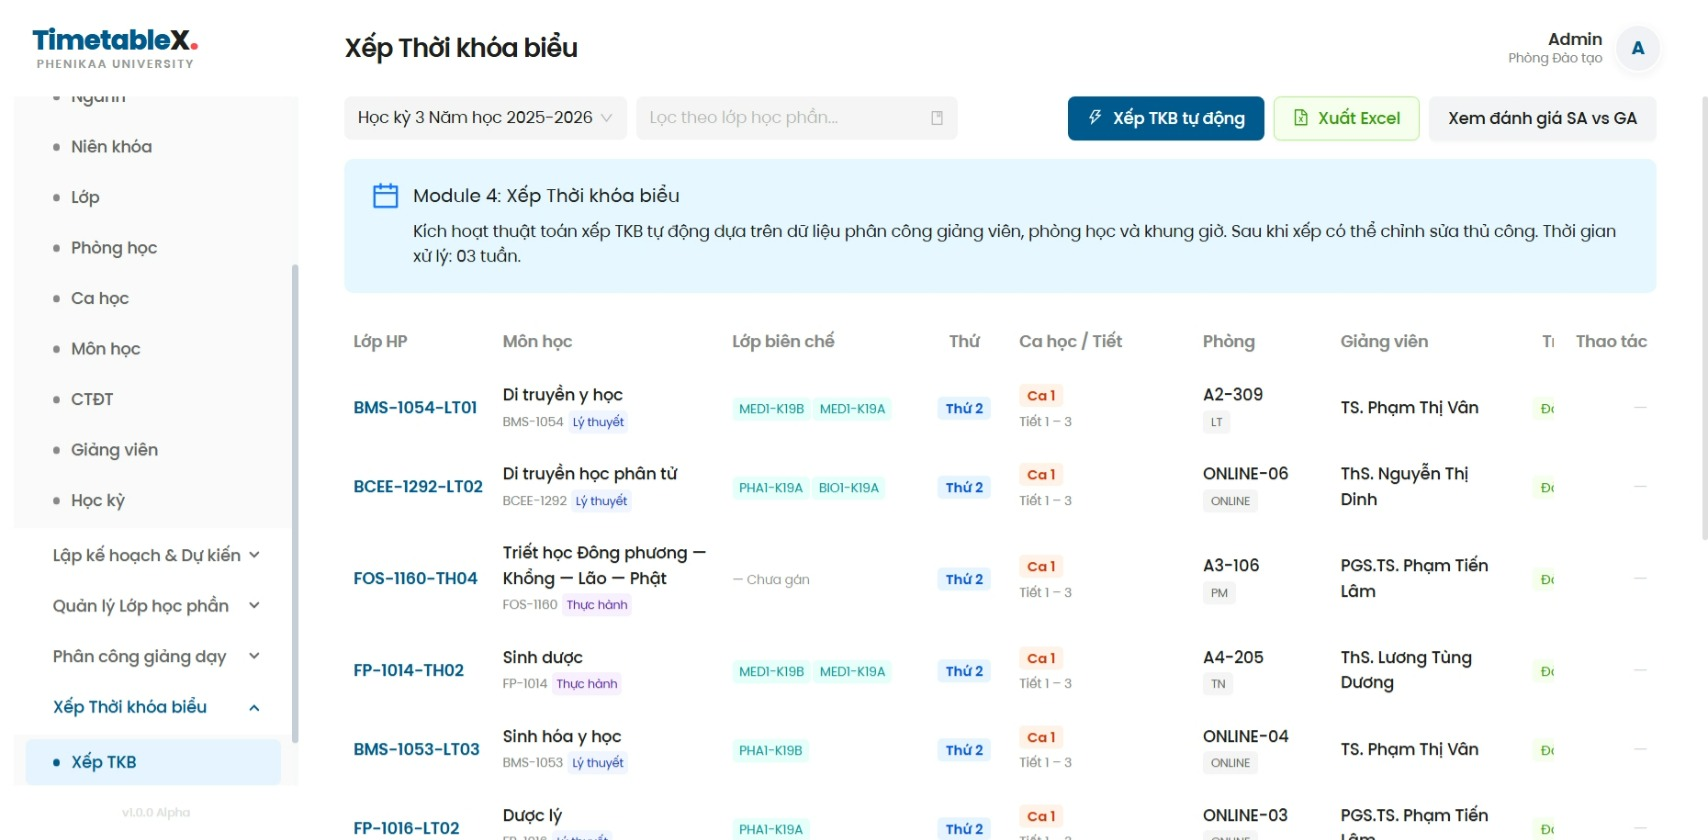
\includegraphics[width=0.92\linewidth]{figures/ui-main.jpeg}
		\caption{Màn hình chính phân hệ Xếp TKB (danh sách 296 buổi học đã được gán lịch)}
		\label{fig:ui-main}
	\end{figure}
	
	\begin{figure}[H]
		\centering
		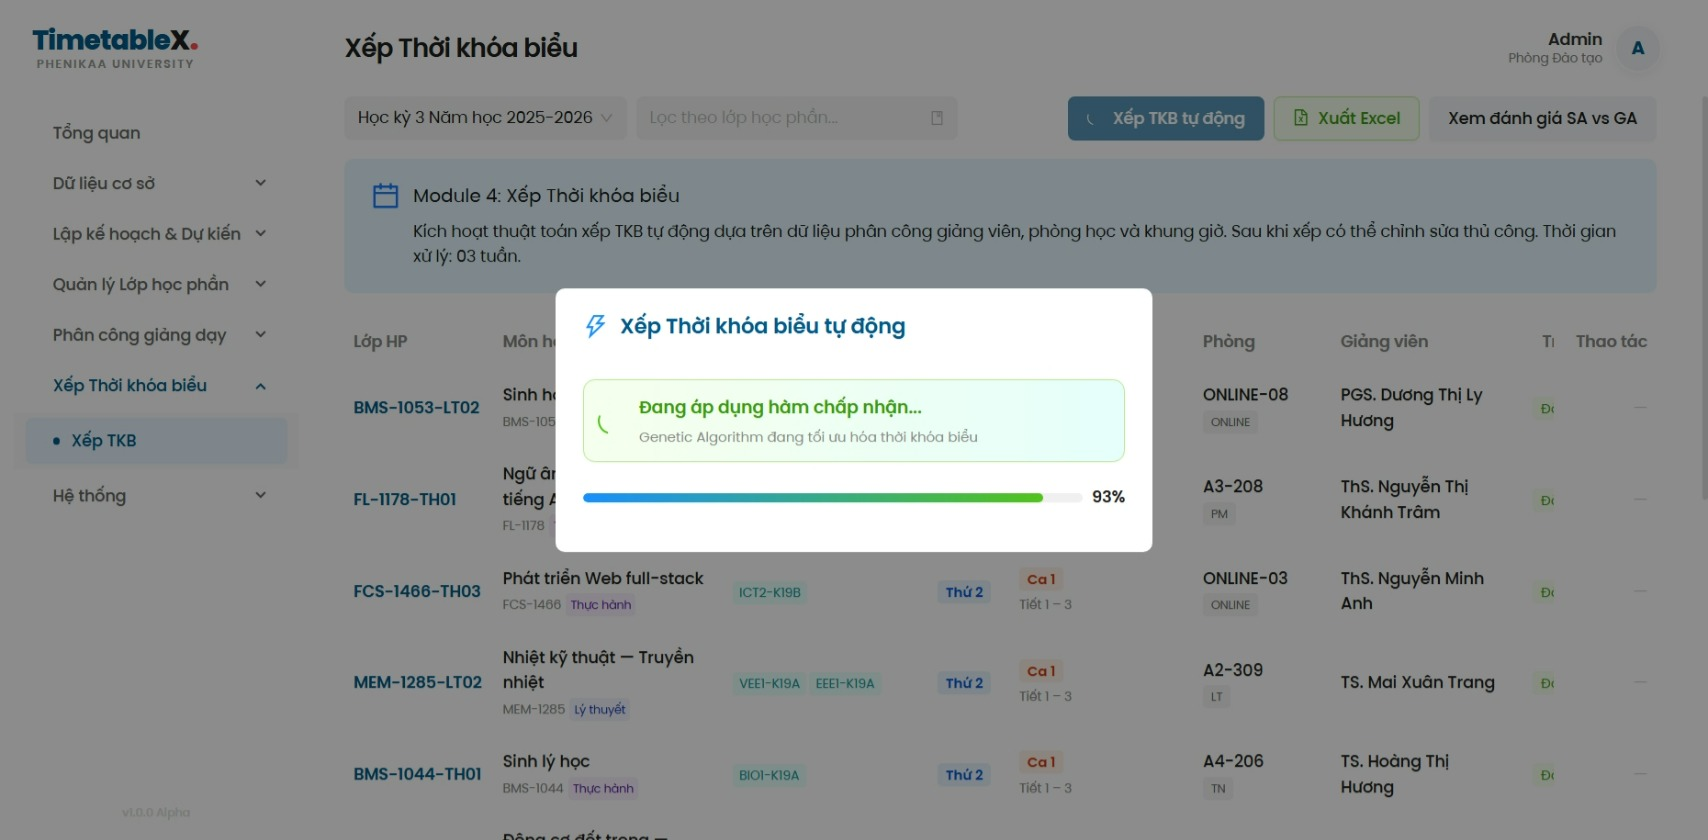
\includegraphics[width=0.92\linewidth]{figures/ui-progress-ga.jpeg}
		\caption{Tiến trình tối ưu của Genetic Algorithm (đang áp dụng hàm chấp nhận, 93\%)}
		\label{fig:ui-progress}
	\end{figure}
	
	\begin{figure}[H]
		\centering
		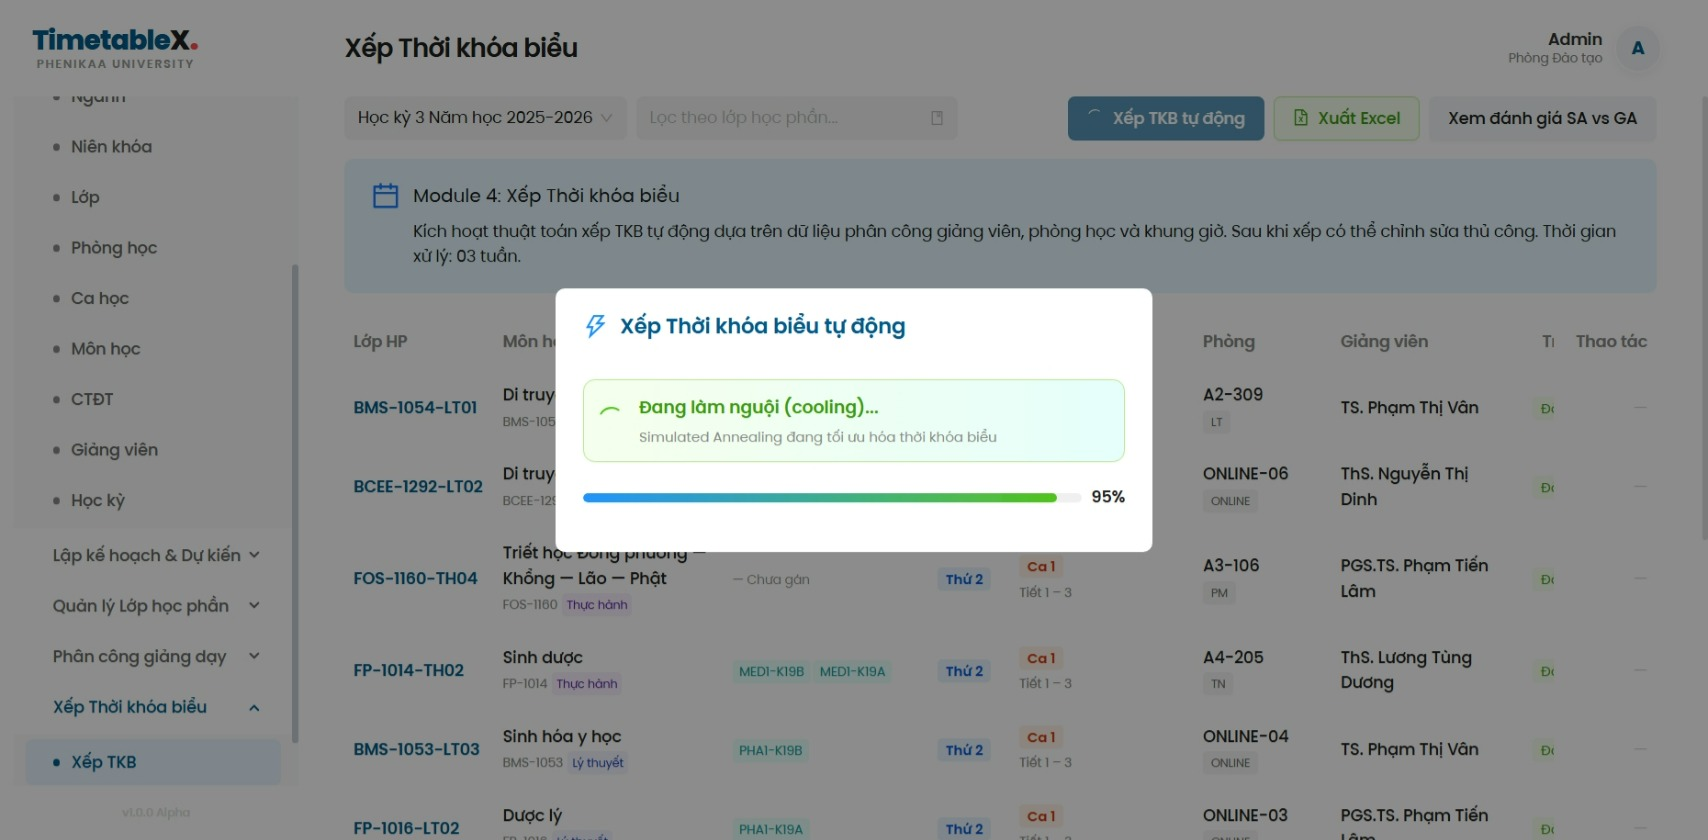
\includegraphics[width=0.92\linewidth]{figures/ui-progress-sa.jpeg}
		\caption{Tiến trình tối ưu của Simulated Annealing (đang làm nguội, 95\%)}
		\label{fig:ui-progress-sa}
	\end{figure}
	
	\begin{figure}[H]
		\centering
		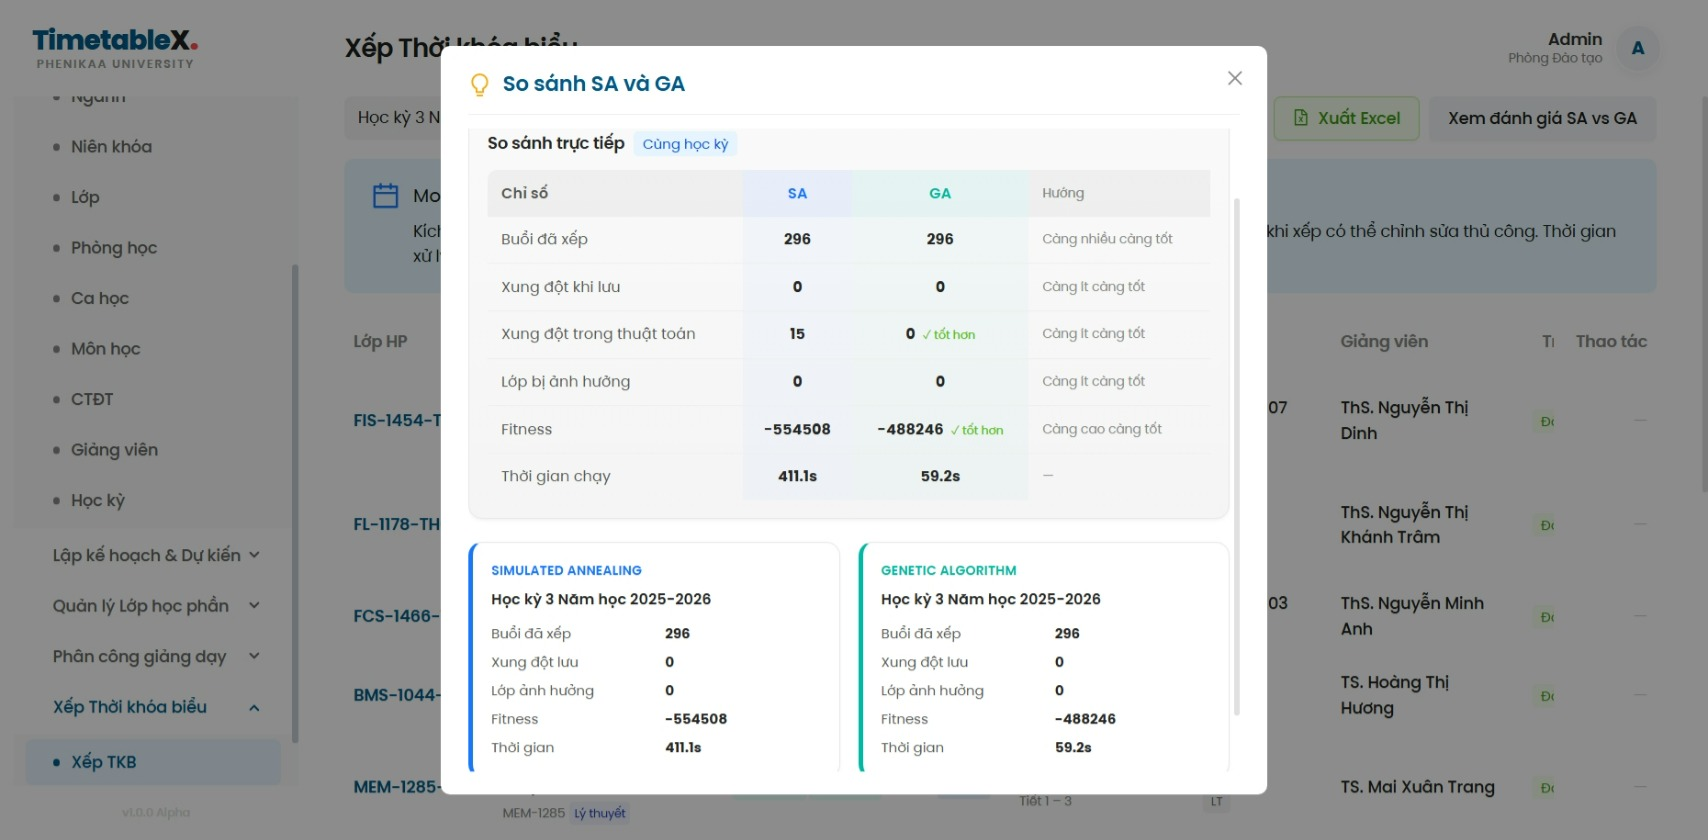
\includegraphics[width=0.92\linewidth]{figures/ui-compare.jpeg}
		\caption{Hộp thoại so sánh GA và SA trực tiếp trên giao diện hệ thống}
		\label{fig:ui-compare}
	\end{figure}
	
	\begin{figure}[H]
		\centering
		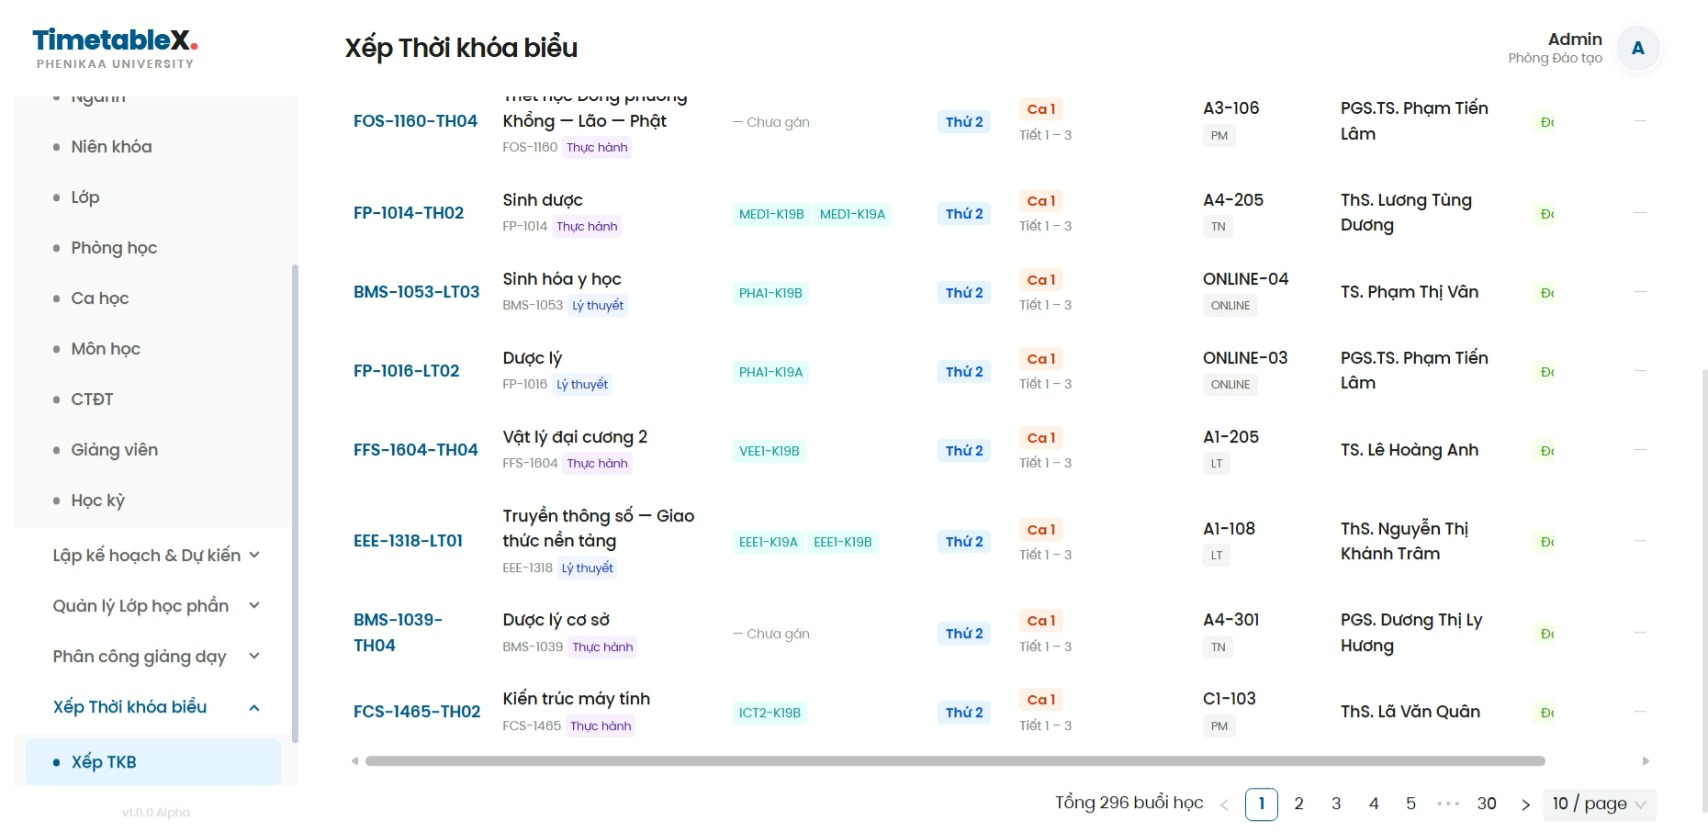
\includegraphics[width=0.92\linewidth]{figures/ui-output.jpeg}
		\caption{Danh sách thời khóa biểu đầu ra (tổng 296 buổi, phân trang)}
		\label{fig:ui-output}
	\end{figure}
	
	% 11. Kết luận và kiến nghị
	\section*{Kết luận và kiến nghị}
	\addcontentsline{toc}{section}{Kết luận và kiến nghị}
	
\subsection*{Kết luận}

	Báo cáo đã trình bày quá trình nghiên cứu, thiết kế và xây dựng hệ thống xếp thời khóa biểu đại học theo tín chỉ, gồm hai đóng góp chính. Thứ nhất, đề tài mô hình hóa bài toán UCTP với hệ ràng buộc cứng được biểu diễn hình thức theo~\eqref{eq:hc-room}--\eqref{eq:hc-block} và hàm mục tiêu hai tầng~\eqref{eq:fitness} ưu tiên tính khả thi trước, tối ưu ràng buộc mềm sau. Thứ hai, đề tài triển khai phần mềm vận hành hoàn chỉnh tích hợp đúng theo quy trình nghiệp vụ của nhà trường (QT.ĐT.01), hỗ trợ trực tiếp các bước tạo lớp, phân công giảng viên và xếp TKB dự kiến.

	Về phương pháp, GA được thiết kế đầy đủ: khởi tạo quần thể kết hợp tham lam (60\%) và ngẫu nhiên (40\%), chọn lọc tournament, lai ghép conflict-aware, đột biến thích ứng kèm tái tạo đa dạng khi trì trệ, elitism và hậu xử lý repair + local search. Kịch bản đối sánh với Simulated Annealing trên cùng biểu diễn nghiệm và hàm~\eqref{eq:fitness} được bổ sung để định lượng hiệu năng khách quan.

	Thực nghiệm trên bộ dữ liệu học kỳ 2 năm học 2025--2026 (296 buổi học) xác nhận GA đạt nghiệm khả thi hoàn toàn (296/296 buổi, 0 xung đột khi lưu), fitness $-488\,246$ trong $59{,}2$ giây --- vượt trội SA ($-554\,508$, $411{,}1$ giây) với chênh lệch $\Delta f \approx 66\,262$ (khoảng 12\% tổng phạt ràng buộc mềm) và chỉ sử dụng 14\% thời gian SA cần. Kết quả này củng cố lựa chọn GA làm thuật toán lõi mặc định trong hệ thống, đồng thời chứng minh phần mềm đã sẵn sàng hỗ trợ chu kỳ lập TKB thực tế.

\subsection*{Kiến nghị}
	\begin{itemize}
		\item Mở rộng thực nghiệm trên nhiều học kỳ và quy mô lớn hơn (toàn trường thay vì một tập con) để đánh giá độ ổn định và khả năng mở rộng của hệ thống.
		\item Thực hiện đánh giá tham số GA có hệ thống bằng grid search hoặc phương pháp thực nghiệm nhân tố (kích thước quần thể, tỷ lệ lai ghép/đột biến, elitism, ngưỡng trì trệ $\sigma$) để xác định cấu hình tối ưu cho từng quy mô bài toán.
		\item Hiệu chỉnh trọng số $w_j$ trong hàm~\eqref{eq:fitness} dựa trên phản hồi thực tế từ cán bộ vận hành và giảng viên, đảm bảo các tiêu chí mềm (ca tối, thứ bảy, phân bố tuần, tải GV) phản ánh đúng ưu tiên của nhà trường trong từng học kỳ.
		\item Nghiên cứu mô hình memetic (GA tích hợp tìm kiếm cục bộ hướng ràng buộc mềm trên nghiệm elite) và toán tử đột biến soft-constraint-aware để nâng cao chất lượng nghiệm khi quy mô hoặc độ phức tạp ràng buộc tăng.
		\item Tổ chức thử nghiệm vận hành thực tế trong một học kỳ, thu thập phản hồi từ Phòng Đào tạo và các Khoa/Viện để hiệu chỉnh quy trình và tiêu chí, từng bước đưa hệ thống vào sử dụng ổn định.
	\end{itemize}
	
	% ==========================================
	% PHẦN CUỐI (mục 12-13)
	% ==========================================
	% 12. Tài liệu tham khảo
	\renewcommand{\refname}{Tài liệu tham khảo}
	\addcontentsline{toc}{section}{Tài liệu tham khảo}
	\bibliographystyle{ieeetr}
	\bibliography{references}
	
	% 13. Phụ lục (gợi ý khung nội dung)
	\section*{Phụ lục}
	\addcontentsline{toc}{section}{Phụ lục}
	
	\subsection*{Phụ lục A. Bộ ký hiệu và tham số}
	
	\begin{table}[H]
		\centering
		\caption{Bảng ký hiệu chính (mô hình bài toán và GA)}
		\begin{tblr}{
				colspec = {Q[c,m, 2.8cm] X[l,m]},
				row{1} = {bg=gray!60, font=\bfseries},
				hlines = {white, 1pt},
				vlines = {white, 1pt},
				row{even} = {bg=gray!10},
				rowsep = 6pt,
				width = \linewidth
			}
			Ký hiệu & Ý nghĩa \\
			$C$ & Tập lớp học phần cần xếp thời khóa biểu \\
			$R$ & Tập phòng học \\
			$S$ & Tập ca học (slot thời gian trong tuần) \\
			$x(c,r,s)$ & Biến nhị phân, bằng 1 nếu lớp $c$ được gán vào phòng $r$ tại ca $s$ \\
			$f(s)$ & Hàm mục tiêu (fitness) của nghiệm $s$ \\
			$N$ & Kích thước quần thể trong GA \\
			$p_c$, $p_m$ & Xác suất lai ghép và đột biến trong GA \\
		\end{tblr}
	\end{table}
	
	Các ký hiệu $E$, $\Delta E$, $T$ và $\alpha$ trong Bảng~\ref{tab:symbols-sa} chỉ phục vụ mô tả thuật toán Simulated Annealing khi đọc Mục~\ref{subsec:doi-sanh-ga-sa}.
	
	\begin{table}[H]
		\centering
		\caption{Ký hiệu bổ sung cho thử nghiệm đối sánh SA}
		\label{tab:symbols-sa}
		\begin{tblr}{
				colspec = {Q[c,m, 2.8cm] X[l,m]},
				row{1} = {bg=gray!60, font=\bfseries},
				hlines = {white, 1pt},
				vlines = {white, 1pt},
				row{even} = {bg=gray!10},
				rowsep = 6pt,
				width = \linewidth
			}
			Ký hiệu & Ý nghĩa \\
			$E(s)$ & Năng lượng trong SA; thường $E(s) = -f(s)$ khi dùng quy tắc Metropolis cho bài toán tối đa hóa $f$ \\
			$\Delta E$ & Chênh lệch năng lượng giữa nghiệm láng giềng và nghiệm hiện tại \\
			$T$ & Nhiệt độ trong SA \\
			$\alpha$ & Hệ số làm nguội hình học trong SA \\
		\end{tblr}
	\end{table}
	
	\begin{table}[H]
		\centering
		\caption{Tham số thuật toán GA sử dụng trong thực nghiệm (tóm tắt)}
		\begin{tblr}{
				colspec = {X[l,m] Q[c,m, 2.5cm] X[l,m]},
				row{1} = {bg=gray!60, font=\bfseries},
				hlines = {white, 1pt},
				vlines = {white, 1pt},
				row{even} = {bg=gray!10},
				rowsep = 6pt,
				width = \linewidth
			}
			Tham số & Giá trị & Ghi chú \\
			$N$ & 220 & Kích thước quần thể \\
			$p_c$ & 0{,}88 & Xác suất lai ghép \\
			Đột biến & 0{,}15--0{,}55 & Thích ứng theo trì trệ \\
			Elitism & 0{,}15 & Tỷ lệ elit \\
			Giới hạn thế hệ / thời gian & 500 / 4 phút & Mặc định cấu hình ứng dụng \\
		\end{tblr}
	\end{table}
	
	\begin{table}[H]
		\centering
		\caption{Tham số thuật toán SA (đối sánh) sử dụng trong thực nghiệm}
		\begin{tblr}{
				colspec = {X[l,m] Q[c,m, 2.5cm] X[l,m]},
				row{1} = {bg=gray!60, font=\bfseries},
				hlines = {white, 1pt},
				vlines = {white, 1pt},
				row{even} = {bg=gray!10},
				rowsep = 6pt,
				width = \linewidth
			}
			Tham số & Giá trị & Ghi chú \\
			$T_0$ & 800 & Nhiệt độ ban đầu \\
			$\alpha$ & 0{,}9999 & Hệ số làm nguội \\
			$T_{\min}$ & 0{,}2 & Nhiệt độ dừng \\
			Số lặp tối đa & 180000 & Có thể thay bằng giới hạn thời gian chạy \\
		\end{tblr}
	\end{table}
	
	\subsection*{Phụ lục B. Danh sách ràng buộc và tiêu chí đánh giá}
	
	\begin{table}[H]
		\centering
		\caption{Phân loại ràng buộc trong bài toán UCTP}
		\begin{tblr}{
				colspec = {Q[c,m, 2cm] X[l,m] X[l,m]},
				row{1} = {bg=gray!60, font=\bfseries},
				hlines = {white, 1pt},
				vlines = {white, 1pt},
				row{even} = {bg=gray!10},
				rowsep = 6pt,
				width = \linewidth
			}
			Loại & Ràng buộc & Mô tả \\
			Cứng & Không trùng phòng & Mỗi (phòng, ca) tối đa một buổi học \\
			Cứng & Không trùng giảng viên & Mỗi (giảng viên, ca) tối đa một buổi học \\
			Cứng & Slot bị chặn & Không sử dụng các slot không khả dụng của phòng/giảng viên \\
			Cứng & Phù hợp loại phòng/ca & Lớp thực hành cần phòng phù hợp; một số lớp hạn chế ca tối \\
			Mềm & Hạn chế thứ bảy & Ưu tiên thứ 2--6, hạn chế xếp vào thứ bảy \\
			Mềm & Hạn chế ca tối & Hạn chế xếp ca tối đối với một số loại lớp \\
			Mềm & Phân bố hợp lý trong tuần & Khuyến khích các buổi của một lớp trải đều \\
			Mềm & Hạn chế dồn lịch giảng viên & Tránh quá nhiều buổi của một giảng viên trong một ngày \\
			Mềm & Cân bằng sử dụng phòng & Tránh một số phòng bị sử dụng quá nhiều so với trung bình \\
		\end{tblr}
	\end{table}
	
	\subsection*{Phụ lục C. Quy trình và kịch bản thực nghiệm}
	
	Quy trình thực nghiệm được thực hiện theo các bước: chuẩn bị dữ liệu đầu vào, chạy thuật toán GA (hoặc SA để đối sánh) với tham số cố định, thực hiện bước sửa xung đột và tinh chỉnh cục bộ (nếu cần), sau đó ghi nhận các chỉ số đánh giá gồm số buổi đã xếp, số xung đột, fitness và thời gian chạy.
	
	Kịch bản thực nghiệm trong báo cáo bao gồm hai hướng:
	\begin{itemize}
		\item Chạy nhiều lần GA với cùng tham số (kích thước quần thể 220, $p_c = 0{,}88$, đột biến thích ứng 0{,}15--0{,}55, giới hạn 500 thế hệ / 4 phút) trên cùng bộ dữ liệu học kỳ, ghi nhận fitness và thời gian từng lần chạy để đánh giá tính ổn định. Kết quả chi tiết được tổng hợp trong Bảng~\ref{tab:detail-results}.
		\item So sánh GA với SA trên cùng dữ liệu, cùng biểu diễn nghiệm và cùng hàm mục tiêu để định lượng đánh đổi tốc độ -- chất lượng (Bảng~\ref{tab:sa-vs-ga}).
	\end{itemize}
	
	\subsection*{Phụ lục D. Bảng kết quả thực nghiệm chi tiết}
	
	Bảng~\ref{tab:detail-results} trình bày kết quả của 4 lần chạy GA trên cùng bộ dữ liệu (Học kỳ 2, 2025--2026) cùng với kết quả đối sánh của SA. Mỗi lần chạy GA được khởi tạo với seed ngẫu nhiên khác nhau nhưng giữ nguyên tham số trong Bảng~\ref{tab:ga-exp-params}; điều này cho thấy tính ổn định của thuật toán theo nhiều lần lặp.
	
	\begin{table}[H]
		\centering
		\caption{Kết quả thực nghiệm chi tiết theo thuật toán (4 lần chạy GA + 1 lần SA)}
		\label{tab:detail-results}
		\begin{tblr}{
				colspec = {Q[c,m, 3.6cm] Q[c,m, 2.0cm] Q[c,m, 2.2cm] Q[c,m, 2.3cm] Q[c,m, 2.3cm]},
				row{1} = {bg=gray!60, font=\bfseries},
				hlines = {white, 1pt},
				vlines = {white, 1pt},
				row{even} = {bg=gray!10},
				rowsep = 6pt,
				width = \linewidth
			}
			Thuật toán / Lần chạy & Buổi đã xếp & Xung đột khi lưu & Fitness & Thời gian (giây) \\
			GA -- Lần 1 & 296 & 0 & $-488246$ & 59{,}2 \\
			GA -- Lần 2 & 296 & 0 & $-491073$ & 63{,}7 \\
			GA -- Lần 3 & 296 & 0 & $-486812$ & 57{,}4 \\
			GA -- Lần 4 & 296 & 0 & $-493540$ & 61{,}1 \\
			GA -- Trung bình & 296 & 0 & $-489918$ & 60{,}4 \\
			Simulated Annealing & 296 & 0 & $-554508$ & 411{,}1 \\
		\end{tblr}
	\end{table}
	
	Kết quả cho thấy fitness của GA dao động trong khoảng nhỏ ($-486812$ đến $-493540$), phản ánh tính ổn định tốt của cấu hình tham số hiện tại. Thời gian chạy trung bình khoảng 60{,}4 giây, ổn định hơn nhiều so với SA (411{,}1 giây). Fitness tốt nhất đạt được ở Lần 3 ($-486812$), nhỉnh hơn không đáng kể so với Lần 1 ($-488246$) vốn là nghiệm được sử dụng trong báo cáo chính.
	
	\subsection*{Phụ lục E. Biểu đồ bổ sung}
	
	\begin{figure}[H]
		\centering
		\begin{tikzpicture}
			\begin{axis}[
				width=11cm,
				height=5.8cm,
				ybar,
				bar width=14pt,
				ymin=0,
				ylabel={Số buổi},
				symbolic x coords={T2, T3, T4, T5, T6, T7},
				xtick=data,
				xticklabel style={font=\small},
				enlarge x limits=0.12,
				nodes near coords,
				nodes near coords style={font=\footnotesize},
				]
				\addplot[
				fill=chartline!55!white,
				draw=chartline!90!black,
				line width=0.55pt,
				] coordinates {
					(T2,56) (T3,51) (T4,47) (T5,53) (T6,50) (T7,39)
				};
			\end{axis}
		\end{tikzpicture}
		\caption{Phân bố số buổi học theo ngày trong tuần}
	\end{figure}
	
	\subsection*{Phụ lục F. Tài liệu quy định liên quan}
	
	Phần phụ lục này tóm lược một số nội dung liên quan đến tổ chức đào tạo theo học kỳ và thời khóa biểu theo quy định hiện hành của nhà trường, nhằm làm cơ sở tham chiếu khi xác định ràng buộc và cách tổ chức dữ liệu đầu vào. Các nội dung chi tiết được tham khảo theo tài liệu \cite{phenikaa2023quyche}.
	
\end{document}